\newpage
%//------ Section 02 -------------------------------------------------------------------------------------------------
\chapter{ALICE: A Large Ion Collider Experiment}
\label{chap:ALICE}
%//-----------------------------------------------------------------------//

As it was already mentionned before, ALICE (\textit{A Large Ion Collider Experiment})  aims at studying QCD bulk matter and, in particular, the quark-gluon plasma (QGP). It is situated in the CERN area, in the vicinity of Geneva, on the ring of the LHC (\textit{Large Hadron Collider}). Being the spearhead of the QGP studies at CERN, it has been designed in order to access to a large variety of observables, able to probe from the initial stage of the collision to the hadron gas phase, over a wide range of transverse momentum.\\

The chapter begins with a brief presentation on CERN in \Sec\ref{sec:CERN}, putting forward the organisational and technical aspects, and most particularly the accelerator complex. Following the same structure, the \Sec\ref{sec:ALICECollaboration} provides a description of the ALICE experiment, from the collaboration to the detector before finishing with the event reconstruction and the offline framework.


\section{The CERN}
\label{sec:CERN}

\subsection{The organisation}


Located the border between France and Switzerland, the CERN is like a tiny country with its own culture, its own language (essentially composed of acronyms). The \fig\ref{fig:CERNView} gives an aerial view of the CERN sites, with an insert on its headquarters in Meyrin (Switzerland, canton of Geneva). It is mostly known for its expertise on particle accelerators and detectors for high energy physics, but it is also the birthplace of some of our everyday devices -- such as the World Wide Web (1990), the touchscreen (1972) -- or less daily tools, like the Worldwide LHC computing grid (2005) and the multi-wire proportionnal chamber (1968). The beginning of the organisation dates back to the 1950s.\\

\begin{figure}[t]
	\centering
	\includegraphics[width=1\textwidth]{Figs/Chapter3/CERN_Final.eps}
	\caption{Aerial view of the CERN accelerator complex (highlighted by the white curves), with an insert on the main site in Meyrin (Switzerland, canton of Geneva). Figure taken from \cite{PuzzleGrandCollisionneur} and modified by the present author.}
	\label{fig:CERNView}
\end{figure}

At the end of the Second World War, Europe lays in ruins, most of the research facilities have been destroyed, many physcists have left the continent to work on the other side of the Atlantic: Europe is no longer at the forefront of scientific progress. A situation from which the old continent might never recover, as the european nations do not have the resources to rebuild the basic infrastucture. Nevertheless, things begin to change in 1949 when, at the European Cultural Conference, Louis de Broglie -- supported by Raoul Dautry, Pierre Auger, Lew Kowarsky, Edoardo Amaldi and Niels Bohr -- proposes to create an European laboratory in order to promote collaboration between Europe's nations, and share the costs.

The project gains momentum such that, in late 1951, the United Nations Educational, Scientific and Cultural Organization (UNESCO) -- pushed by the United States -- organises a dedicated meeting on that matter. Some countries shows their skepticism. This is not surprising: even though the infrastructure costs are mutualised, this kind of endeavor still demands an initial investement, many countries are in a difficult financial position and are thus reluctant to participate. After two months of debate, the first resolution of the convention establishing the European Council for Nuclear Research ("Conseil Européen pour la Recherche Nucléaire" in French or CERN) is ratified in 1952 by the twelve founding member states: Belgium, Denmark, France, Germany, Greece, Italy, Netherlands, Norway, Sweden, Switzerland, United-Kingdom and Yugoslavia \cite{deroseParis1951Birth2008}.

Later that year, Geneva was chosen to host the laboratory. In 1953 the CERN convention is completed and signed by all the members. It defines, amongst others, the membership, the financial contributions, the decision protocols, its denomination\footnote{The CERN Convention was the opportunity to rename the CERN as the "Organisation Européenne pour la Recherche Nucléaire" (or European Organisation for Nuclear Research in English), that would corresponds to the acronym OERN now. Because the initial abbreviation turns out to be more elegant, the CERN remained.} and its missions. In particular, the CERN aims not only for technological developments and scientific research on high-energy physics but also for the "promotion of contacts between, and the interchange of, scientists, the dissemination of information [...]", and "collaborating with and advising other research institutions" \cite{cerncouncilConventionEstablishmentEuropean1953}.\\

Nowadays, the organisation includes 23 Member States and ten Associate Member States. There are also non-members States or institution with an Observer status, such as the United-States, Japan, European Union, UNESCO and formerly the Russian Federation. In 2017, the CERN counted more than 17 500 people, all over the world, working together towards a common goal, including more than 12 200 scientists\cite{cernOurPeople2023}. This makes it the largest scientific organisation in the World.

\subsection{The accelerator complex}
\label{subsec:AcceleratorComplex}

As stated in the Article II of the Convention, the construction and operation of particle accelerators stand as one of the CERN's purposes. In particular, the organisation must immediately develop a 600 \mev synchro-cyclotron and a 28 \gev proton synchrotron (PS). The former, built in 1957, corresponds to the first accelerator of CERN; the latter starts accelerating protons in 1959.

The next step up in beam energies arrives in 1976 with the first underground accelerator, the Super Proton Synchroton (SPS). It consists in two rings, of seven kilometers circumference each, delivering beams of 300 \gev of protons and antiprotons. At least, on the paper because it is one of the rare cases in particle physics, when the final product performs better than expected in the technical design reports. Thanks to technological advances during its construction, the SPS could reach beam energies up to 400 \gev, and gradually of 450 \gev after some upgrades.

In 1989, a 27-kilometre circular accelerator enters in operation, namely the Large Electron-Positron (LEP) collider. It was tuned such that the colliding energy sits on the resonance mass peak of the \rmZzero and \rmWplusminus bosons, but in the search of the Higgs boson, it was operated with a centre-of-mass energy of 209 \gev on its last year, in 2000. This was -- and still is -- the largest electron-positron collider ever built.

As one World record calls for another, the LEP collider is decomissionned in order to be replaced in 2008\footnote{Technically, because of an incident on one of the dipole magnets, the accelerator undergoes some repairs that delay its operation by fourteen months.} by the Large Hadron Collider (LHC), the World's largest and most energetic particle collider. The accelerator is currently operational and should still be, at least, until 2038. Beyond this date, the CERN might start the construction of the Future Circular Collider, a particle accelerator with a circumference of 100 km\cite{FutureCircularCollider2023}\cite{benediktFutureCircularCollider2019}.\\

\begin{table}[!h]
    \centering
    \begin{tabular}{p{5.5cm}@{\hspace{1cm}} p{2.25cm}@{\hspace{0.75cm}} p{2.25cm}@{\hspace{0.75cm}} p{2.25cm}@{}}
    \noalign{\smallskip}\hline\noalign{\smallskip}
    Collision type & pp & Pb-Pb & Xe-Xe \\
    Energy per beam & 6.5 \tev & 2.56 \tev & 2.72 \tev \\
    Luminosity ($cm^{-2} s^{-1}$) & $2.1 \times 10^{34}$ & $6.1 \times 10^{27}$  & $0.4 \times 10^{27}$ \\
    Velocity (in units of $c$) & 0.99999998 & 0.99715693 & 0.99898973 \\
    \noalign{\smallskip}\hline \noalign{\smallskip}
    Circumference & \multicolumn{3}{c}{26 659 m} \\
    Beam vacuum & \multicolumn{3}{c}{$10^{-13}$ atm} \\
    Number of RF cavities & \multicolumn{3}{c}{8 per beam} \\
    Number of magnets & \multicolumn{3}{c}{9593} \\
	Number of dipole magnets & \multicolumn{3}{c}{1232}\\
	Dipole operating temperature & \multicolumn{3}{c}{1.9 K (-271.3 C)}\\
	Current flowing in the dipole & \multicolumn{3}{c}{11 850 A}\\
	Magnetic field of the dipole & \multicolumn{3}{c}{8.33 T}\\
    \noalign{\smallskip}\hline\noalign{\smallskip}
    \end{tabular}
    \caption{A selection of design parameters for the LHC during the Run-2. Values taken from \cite{LHCGuide2017} and \cite{particledatagroupReviewParticlePhysics2022}.}\label{tab:LHCCharacteristics}
\end{table}

The LHC is the collider of (almost) all superlatives. To put it into perspectives, the \tab\ref{tab:LHCCharacteristics} lists some of its important characteristics. 

As in any accelerator, particles circulate in a vacuum tube in order to avoid collisions with gas molecules. The beam is subject to ultra-high vacuum, corresponding to a pressure of $10^{-13}$ atm, applied over the approximately 9 000 $m^{3}$ covered by the LHC. In comparison, this is like pumping down the nave of a cathedrale to a pressure level similar to the one on the Moon. 

The particle trajectory is controlled by various magnets: 1232 dipoles to bend the 6.5 \tev beams, 392 quadrupoles to squeeze and focus the beam down to the collision point, etc. If we hope to curve the particle's trajectory at the LHC energies, the dipoles must create an intense magnetic field of 8.33 T, demanding a current of 11 850 A. At ambient temperature, the dissipated heat would melt down the magnet. For that reason, 90 tonnes of superfluid helium are injected into the magnets bringing their temperature down to 1.9 K (-271.3 C), that is even lower than the temperature of outer space (2.7 K). At this level, the dipoles become superconducting and can now bear the flow of currents to develop the necessary magnetic field. 

The particle acceleration is ensured by eight radiofrequency cavities (RF cavities)\footnote{It consists in a cavity filled with an electromagnetic field oscillating at a specific frequency (in the radio wave's domain, hence the name of the radiofrequency cavities), and shaped in such a way that resonance occurs.} per beam. Most often, they accelerate protons at 6.5 \tev, which corresponds to the typical kinetic energy of flying mosquito but distributed on the minuscule volume of a proton. At such energy, a proton travels at almost light-speed and makes 11 245 LHC turns per second. As a consequence of the RF cavities, each beam is divided into 2808 bunches separated by 7.5 m (or 25 ns\footnote{This is the case for the LHC Run-2, but in the Run-1, the distance between two bunches was twice as big, that is 50 ns.}) and containing about $10^{11}$ protons. \\

\begin{figure}[t]
	\centering
	\includegraphics[width=1\textwidth]{Figs/Chapter3/CCC-v2022_Large.png}
	\caption{Schematic representation of the CERN accelerator complex as in 2023. Figure taken from \cite{lopienskaewaCERNAcceleratorComplex2022}.}
	\label{fig:AcceleratorComplex}
\end{figure}

It is noteworthy that the LHC is only the last element of the acceleration chain, as represented in the \fig\ref{fig:AcceleratorComplex}. The beam energy increases gradually using the past CERN's accelerators. Depending on the type of beams (pp or AA), the route to the LHC differs slightly. For a proton beam, negatively charged hydrogen ions are first accelerated by the Linear Accelerator 4 (LINAC 4)\footnote{Until 2020, the first acceleration stage was performed by the LINAC 2 that accelerated hydrogen atoms.} to 160 \mev, and then they are injected in the Proton Synchroton Booster (BOOSTER) in order to reach an energy of 2 \gev. The electrons of the hydrogen ions are removed when leaving the LINAC 4. For a heavy-ion collision, the Linear Accelerator 3 (LINAC 3) provides a beam of heavy-ions -- already stripped of their electrons -- to the Low Energy Ion Ring (LEIR), which accelerates them to 72 \mev per nucleon. Whether it is a beam made of protons or heavy-ions, they are successively accelerated by the PS and SPS up to 450 \gev (or 177 \gev per nucleon for heavy-ions). The particles are finally injected in the rings of the LHC in order to reach their top energy of 6.5 \tev (or 2.56 \tev per nucleon for Pb beams) and collide in the four collision points where sits the four main LHC's experiments: ATLAS, CMS, LHCb, and ALICE\cite{AcceleratorComplexCERN}. \Tab\ref{tab:LHCExperiments} presents a few of their characteristics. 

\begin{table}[!h]
    \centering
    \begin{tabular}{p{3cm}@{\hspace{1cm}} p{2cm}@{\hspace{0.75cm}} p{2cm}@{\hspace{0.75cm}} p{2cm}@{\hspace{0.75cm}} p{2cm}@{}}
    \noalign{\smallskip}\hline\noalign{\smallskip}
    Experiment & ATLAS & CMS & ALICE & LHCb\\
    \noalign{\smallskip}\hline \noalign{\smallskip}
    Participants & 5 991 & 5 824 & 2 085 & 1 585\\
    \noalign{\smallskip}\hline \noalign{\smallskip}
    Height (m) & 25 & 15 & 16 & 10\\
    Length (m) & 46 & 21 & 26 & 21\\
    Width (m) & 25 & 15 & 16 & 13\\
    Weight (tonnes) & 7 000 & 14 000 & 10 000 & 5 600\\
    \noalign{\smallskip}\hline\noalign{\smallskip}
    \end{tabular}
    \caption{A few characteristics of the four main LHC experiments, namely ATLAS, CMS, ALICE and LHCb. The participants include particle physicists, engineers, technicians and students; their number corresponds to the one as of March 2023\cite{Greybook}. The dimensions of each detector originate from \cite{aadATLASExperimentCERN2008}\cite{cmscollaborationCMSExperimentCERN2008}\cite{alicecollaborationALICEExperimentCERN2008}\cite{lhcbcollaborationLHCbDetectorLHC2008}.}\label{tab:LHCExperiments}
\end{table}

A Toroidal LHC Apparatus (ATLAS) and a Compact Muon Solenoid (CMS) are the most colossal experiments at the LHC, as much in terms of the number of participants as in the dimension of their detectors. Both cover a wide range of physics and share the same goals, namely characterising the elementary particles of Standard Model -- in particular, the Higgs boson -- and searching for the new particles beyond the Standard Model, such as dark matter candidates or supersymmetric particles. 

ALICE and LHCb (Large Hadron Collider beauty) are more specialised. ALICE aims at studying QCD matter, and particularly under extreme energy densities where a phase of deconfined quark-gluon matter forms, the QGP. On the other hand, LHCb focuses on heavy flavour physics. It is concerned about new physics in the CP violation and rare decays of primarily beauty but also charm hadrons.\\

In order to carry out their physics programme, the LHC must provide different types of beam. For instance, ATLAS and CMS are essentially interested in pp collisions with the highest interaction rate possible, whereas ALICE needs heavy-ion runs to study \textit{directly}\footnote{As discussed in \Sec\ref{subsec:ComparisonPP}, the QGP can also be investigated via the study of its signatures in pp collisions.} the QGP. Therefore, the Run Coordination of each experiment gathers regularly with LHC Programme Coordination to discuss -- and even negotiate -- the accelerator schedule and define a programme which best meets everyone's needs.

\subsection{The accelerator programme}

\begin{table}[!t]
    \centering
    \begin{tabular}{b{2cm}@{\hspace{0.5cm}} b{1cm}@{\hspace{0.75cm}} b{1.5cm}@{\hspace{0.75cm}} b{2.5cm}@{\hspace{0.25cm}} >{\raggedleft\arraybackslash}b{5cm}@{\hspace{0.25cm}}}
    \noalign{\smallskip}\hline\noalign{\smallskip}
    LHC Run & Year & Collision & Centre-of-mass energy (per nucleon) & Dates \\
    \noalign{\smallskip}\hline \noalign{\smallskip}
    \bf Run 1 & 2009 & pp & 900 \gev & 23$^{\textrm{rd}}$ Nov. to 14$^{\textrm{th}}$ Dec.\\
     & & pp & 2.36 \tev & 14$^{\textrm{th}}$ and 16$^{\textrm{th}}$ Dec.\\
    \\
     & 2010 & pp & 7 \tev & 30$^{\textrm{th}}$ Mar. to 4$^{\textrm{th}}$ Nov.\\
     &  & pp & 900 \gev & 2$^{\textrm{nd}}$, 3$^{\textrm{rd}}$ and 27$^{\textrm{th}}$ May\\
     &  & Pb-Pb & 2.76 \tev & 9$^{\textrm{th}}$ Nov. to 6$^{\textrm{th}}$ Dec.\\
     \\
    
     & 2011 & pp & 7 \tev & 21$^{\textrm{th}}$ Feb. to 4$^{\textrm{th}}$ Nov.\\
     &  & pp & 2.76 \tev & 24$^{\textrm{th}}$ to 27$^{\textrm{th}}$ Mar.\\
     &  & Pb-Pb & 2.76 \tev & 5$^{\textrm{th}}$ Nov. to 7$^{\textrm{th}}$ Dec.\\
     \\
     & 2012 & pp & 8 \tev & 5$^{\textrm{th}}$ Apr. to 16$^{\textrm{th}}$ Dec.\\
     \\
     & 2013 & p-Pb & 5.02 \tev & 20$^{\textrm{th}}$ Jan. to 10$^{\textrm{th}}$ Feb.\\
     & & pp & 2.76 \tev & 11$^{\textrm{th}}$ to 14$^{\textrm{th}}$ Feb.\\
     
    \noalign{\smallskip}\hline \noalign{\smallskip}
    
	\bf Run 2 & 2015 & pp & 13 \tev & 3$^{\textrm{rd}}$ Jun. to 19$^{\textrm{th}}$ Nov.\\
     & & pp & 5.02 \tev & 19$^{\textrm{th}}$ to 23$^{\textrm{rd}}$ Nov.\\
     & & Pb-Pb & 5.02 \tev & 24$^{\textrm{th}}$ Nov. to 13$^{\textrm{th}}$ Dec.\\
    \\
     & 2016 & pp & 13 \tev & 23$^{\textrm{rd}}$ Apr. to 26$^{\textrm{th}}$ Oct.\\
     &  & p-Pb & 5.02 \tev & 4$^{\textrm{th}}$ to 17$^{\textrm{th}}$ Nov.\\
     &  &  &  & 4$^{\textrm{th}}$ to 5$^{\textrm{th}}$ Dec.\\
     &  & p-Pb & 8.16 \tev & 18$^{\textrm{th}}$ to 25$^{\textrm{th}}$ Nov.\\
     &  & Pb-p & 8.16 \tev & 26$^{\textrm{th}}$ Nov. to 4$^{\textrm{th}}$ Dec.\\
    \\
     & 2017 & pp & 13 \tev & 23$^{\textrm{rd}}$ May to 26$^{\textrm{th}}$ Nov.\\
     &  & pp & 5.02 \tev & 11$^{\textrm{th}}$ to 21$^{\textrm{st}}$ Nov.\\
     &  & Xe-Xe & 5.44 \tev & 12$^{\textrm{th}}$ Oct.\\
     \\
     & 2018 & pp & 13 \tev & 12$^{\textrm{th}}$ Apr. to 23$^{\textrm{th}}$ Oct.\\
     &  & Pb-Pb & 5.02 \tev & 7$^{\textrm{th}}$ Nov. to 2$^{\textrm{nd}}$ Dec.\\
    \noalign{\smallskip}\hline\noalign{\smallskip}
    \end{tabular}
    \caption{Summary of the LHC Run 1 and 2 physics programmes with the data taking periods in the rightmost column \cite{LHCCommissioning}.}\label{tab:LHCRunProgramm}
\end{table}

The LHC delivers his first collisions on the 23$^{\textrm{rd}}$ of November 2009; these are pp collisions at \sqrtS = 900 \gev. The centre-of-mass energy gradually increases over the years, from 0.9 \tev to 2.36 and then 7 \tev in 2011, and 8 \tev in 2012. The proton-proton programme is complemented by Pb-Pb collisions at \sqrtSnn = 2.76 \tev in November 2010 and 2011, followed in early 2013 by the first p-Pb run at a centre-of-mass energy per nucleon of 5.02 \tev. A few days later, the collider enters in a long shutdown (LS1), marking the end of the first campaign of data taking now called Run-1 (2009-2013). During this period, the LHC undergoes maintenance operations and preparations in view of an increase by a factor two of both energy (reaching \sqrtS = 13 \tev in pp collisions) and luminosity\footnote{This quantity corresponds to a measure of the number of collisions either per unit of time (\textit{instantaneous luminosity}) or over a certain period of time (\textit{integrated luminosity}). In the latter case, it is expressed in inverse barns (\invb) or femtobarns (\invfb).} (bunches of protons are separated by 25 ns instead of 50 ns).

In spring 2015 begins the second campaign of data taking, the LHC Run-2. The latter opens with pp collisions at a record energy of 13 \tev, which will be the default collisional energy in pp until the end of the Run-2. The same goes for heavy-ion collisions: the Pb-Pb and p-Pb data are now collected at \sqrtSnn = 5.02 \tev, and up to 8.16 \tev in the latter case. Note also the presence of a short Xe-Xe run at \sqrtSnn = 5.44 \tev in October 2017. The Run-2 comes to an end on December 2018; the LHC enters in its second long shutdown (LS2). As for the LS1, this is the opportunity for the collider and its experiments to be renovated and upgraded. 

On the 5th of July 2022, the LHC restarts and delivers its first pp collisions -- almost four years after the start of the LS2 -- at the new record energy of 13.6 \tev, signalling the beginning of the Run-3.

\section{The ALICE collaboration}
\label{sec:ALICECollaboration}

Amongst the different collaboration based at CERN, ALICE holds a particular place since the work presented in this manuscript has been realised within this experiment. As mentionned above, it aims at studying the properties of strongly interacting matter and particularly under extreme energy densities where the quark-gluon plasma is formed (\Sec\ref{sec:QGP}). 

\subsection{The collaboration}

As of March 2023, the ALICE collaboration counts 2084 physicists, engineers, technicians and students from 174 institutes in 41 countries. Most of its members originate from Europe (France, Italy, Germany,...), but also from Asia (China, South Korea, Japan,...) and America (United States, Brazil, Mexico,...). In order to coordinate the efforts within the collaboration, ALICE is organised in different boards and committees, each covering a specific scope\footnote{Only a subset of the ALICE management structure is mentionned. The complete picture is specified in the ALICE Constitution \cite{alicecollaborationALICECollaboration}.}:

\begin{itemize}
\item[$\bullet$] \textit{The Collaboration Board (CB)} is the highest body of collaboration, it can examine and render a decision on any issues from the construction of the detector to the publication policy. It consists in a legislative assembly, mainly composed of the representatives of each member institute (one per member).
\item[$\bullet$] \textit{The Management Board (MB)} supervises the experiment in any matters (scientific, technical, organisational, operational and financial). It plays the role of the executive authority of the collaboration, and is represented by the Spokesperson and its deputies.
\item[$\bullet$] \textit{The Resource Board (RB)} deals with the financial aspect of ALICE. Each national funding agency has a seat within this committee.
\item[$\bullet$] \textit{The Physics Board (PB)} coordinates the analysis work in order to address the physics goals defined by the CB and MB. It consists in eight Physics Working Groups (PWG), each covering a specific theme, as presented in \tab\ref{tab:PhysicsBoard}.

\begin{table}[h]
    \centering
    \begin{tabular}{p{5cm}@{\hspace{0.5cm}} >{\raggedright\arraybackslash}p{7cm}@{\hspace{0.5cm}}}
    \noalign{\smallskip}\hline\noalign{\smallskip}
	Physics Working Group & Topic\\
    \noalign{\smallskip}\hline \noalign{\smallskip}
    \textit{PWG-CF} & Correlations and Flow\\
	\textit{PWG-DQ} & Dileptons and Quarkonia\\
	\textit{PWG-EM} & Electromagnetic probes\\
	\textit{PWG-HF} & Heavy Flavour\\
	\textit{PWG-JE} & Jets\\
	\textit{PWG-LF} & Light-Flavours\\
	\textit{PWG-MM} & Monte Carlo generators and Minimum bias analysis\\
	\textit{PWG-UD} & Ultra-peripheral collisions and Diffraction\\
    \noalign{\smallskip}\hline\noalign{\smallskip}
    \end{tabular}
    \caption{The eight working groups of the ALICE Physics Board, as of 2023.}\label{tab:PhysicsBoard}
\end{table}

Each PWG is also subdivided in Physics Analysis Group (PAG). For instance, the PWG-Light Flavours includes four PAGs: \textit{Resonances}, \textit{Spectra}, \textit{Nuclei and Exotica}, and \textit{Strangeness}. The present analyses on multi-strange baryons (\chap\ref{chap:CPTAnalysis} and \ref{chap:CorrelatedAnalysis}) are part of the latter group.

\item[$\bullet$] \textit{The Run Coordination (RC)} is responsible for the operation of the ALICE detector. Amongst its duties, it must ensure efficient data taking, optimal data quality and must define the LHC schedule with the LHC Programme Coordination in order to meet the physics goals of the collaboration.
\item[$\bullet$] \textit{The Editorial Board (EB)} manages the publication process (publication, conference proceedings, internal and technical notes). It is complemented by the \textit{Conference Committee (CC)} that oversees the oral presentations (talk or poster) outside of the collaboration.
\end{itemize}

This structure is quite common in high-energy experiments, most of the collaboration being organised in this way. With different denominations perhaps, but the essence stays the same.

\subsection{The detector}
\label{subsec:ALICEDetector}

The ALICE detector sits in a cavern 56 m below the ground, in the vicinity of Saint-Genis-Pouilly in France. It is located at the interaction point 2 of the LHC, where the L3 experiment at the former LEP collider was installed. From the latter only remains the gigantic red octogonal solenoid magnet, now symbol of the ALICE collaboration.

Being the only experiment dedicated to studying the QGP, ALICE has been designed as general-purpose detector capable of accessing a large number of observables. The physics targets impose several design constraints.

\begin{figure}[!t]
	\centering
	\includegraphics[width=0.85\textwidth]{Figs/Chapter3/ALICE_PID_performance_v3.eps}
	\caption{ALICE particle identification and reconstruction as a function of \pT. Figure taken from \cite{alicecollaborationALICEExperimentJourney2022}.}
	\label{fig:PIDCapabilities}
\end{figure} 

The apparatus must be able to operate in a high-multiplicity environment, considering that the charged particle density per unit of rapidity in the most violent Pb-Pb collisions may reach $\dNchdeta = 2035 \pm 52$ \cite{alicecollaborationCentralityDependenceChargedParticle2016}. For that reason, high granularity detectors -- such as the Inner Tracking System -- are employed to ensure an excellent reconstruction of the primary and secondary vertices, especially close to the interaction point. In fact, the design of ALICE was optimized to endure values up to $\dNchdeta = 4000$, and twice as much in simulations.

To gain as much insights as possible on the QGP evolution, most of the measurements shall be achievable over a wide momentum range, spanning from very low transverse momentum ($\sim$100 \mmom) -- where most of the particle production is -- up to large transverse momentum ($\geq$ 100 \gmom). This requires reducing the multiple scattering at low \pT, and thus using extremely thin detectors. The material budget amounts at central rapidity to 13\% radiation length, \Xzero\footnote{This is the characteristic amount of matter over which a high-energy electron loses all its energy by bremsstrahlung (\ie deceleration via the emission of photons) but 1/$e$. It is expressed in g.cm$^{-2}$ \cite{particledatagroupReviewParticlePhysics2022}.}, up to Time Projection Chamber outter wall\footnote{Here, there are two antogonistic constraints: the detectors must be thin and radiation tolerant in order to function in a high-multiplicity environment, the latter requiring relatively thick materials. However, in ALICE, the interaction rate in heavy-ion collisions is low (about 10 kHz or 10 000 Pb-Pb collisions per second) such that the radiation doses are rather mild, compared with the levels in ATLAS and CMS (790 and 840 kGy respectively): the total dose over the period of a LHC-Run varies between tens of Gy for the furthest parts of the Inner Tracking System to 2.7 kGy close to the interaction point.}. For comparison, it is about 47\% and 40\% \Xzero in ATLAS and CMS at the end of their inner tracker \cite{aadATLASExperimentCERN2008}\cite{cmscollaborationCMSExperimentCERN2008}, and 17.5\% \Xzero down to the VELO (VErtex LOcator) for LHCb \cite{lhcbcollaborationLHCbDetectorLHC2008}. At high \pT, the constraint lies in the need for a good resolution at large transverse momentum. This is achieved by means of a large tracking lever arm thanks to the Time Projection Chamber, that extends up to 2.5 m. 

That brings an extra consideration. In order to avoid excessivily bending the low \pT charged particles and making them impossible to detect, the momentum measurement down to 100 \mmom necessitates a moderate magnetic field of 0.5 T\footnote{Among the four main LHC experiments, this is the most moderate magnetic field. For comparison, CMS uses a magnetic field of 4 T, the same as the LHCb dipole magnet, and ATLAS solenoid magnet delivers a 2 T field.}. In return, the high \pT charged particles are less curved resulting in a reduction of the momentum resolution, when they are still measurable. 

Along the same line, many observables depend on the nature of the particle, and so it is essential to have a robust particle identification (PID) over a wide momentum range. To that end, ALICE exploits all the PID techniques on the market: ionization energy loss in the Time Projection Chamber, time-of-flight measurement with the Time-Of-Flight detector, Cerenkov and transition radiations in the High-Momentum Particle Identification Detector and Transition Radiation Detector respectively, energy measurement with the Electromagnetic Calorimeters and the Photon Spectrometer. The \fig\ref{fig:PIDCapabilities} provides an overview of the PID and reconstruction capabilities with the transverse momentum coverage.\\


\Fig\ref{fig:ALICEdetector} provides a overview of the different elements of the detector. It comprises 19 detection systems organised in two groups: the ones in the central barrel at mid-rapidity ($|\eta| < 0.9$), embedded in the L3 solenoid magnet that delivers a homogenous magnetic field up to 0.5 T; the others at forward rapidity ($-4 < \eta < -2.5$), dedicated to muon detection. An exhaustive description of the ALICE apparatus can be found in \cite{alicecollaborationALICEExperimentCERN2008}, as well as its physics performances in \cite{carminatiALICEPhysicsPerformance2004}\cite{alicecollaborationALICEPhysicsPerformance2006}\cite{alicecollaborationPerformanceALICEExperiment2014}. In the next paragraphs, we will concentrate on the main detectors employed in this thesis, namely the Inner Tracking System (\ref{subsubsec:ITS}), the Time Projection Chamber (\ref{subsubsec:TPC}), the VZERO (\ref{subsubsec:VZERO}) and the Time-Of-Flight detector (\ref{subsubsec:TOF}). 

Before proceeding, a note on the location of the different parts of the apparatus: in the cartesian coordinate system of ALICE, the origin lies at the centre of the central barrel and the $z$-axis coincides with the beams. The elements located on positive $z$ belongs to the A-side (Anti clockwise, beam going from ALICE to the ATLAS interaction point), the others with negative $z$ are on the C-side (Clockwise, beam going from ALICE to the CMS interaction point). The $y$-axis points towards the top of the detector and the $x$-axis is in the horizontal plane, going towards the centre of the LHC ring. Moreover, there exists a cylindrical coordinates system based on the distance from the origin $r$ and the azimuthal angle $\varphi$ in the transverse plane $xy$, as well as a spherical one with an additional angle, the zenithal angle denoted $\theta$.


\begin{figure}[t]
	\centering
	\includegraphics[width=1\textwidth]{Figs/Chapter3/ALICE.png}
	\caption{Schematic representation of the ALICE apparatus, as it was operated in the LHC Run-2. Figure taken from \cite{alicecollaborationALICEExperimentJourney2022}.}
	\label{fig:ALICEdetector}
\end{figure}


\subsubsection{Inner Tracking System}
\label{subsubsec:ITS}

The Inner Tracking System (ITS) of ALICE is the closest detection system to the interaction point. It surrounds the beam pipe, a 800 \mum-thick beryllium cylinder with a radius of 2.9 \cm. The ITS is designed in order to i) estimate the primary vertex position to a precision better than 100 \mum, ii) reconstruct secondary decay vertices of relatively short lifetime particles such as hyperons, D or B mesons, iii) track and identify particles whose $\pT \leq 200 \mmom$, iv) bring constraints on the particles reconstructed by the Time Projection Chamber and, by so doing, improve the momentum and angle resolution, v) enhance PID capabilities of the ALICE apparatus, and finally vi) provide additionnal trigger information. As shown on the \fig\ref{fig:ITSstructure}, the ITS is made of six coaxial cylindrical layers of silicon detectors based on three different technologies. The two innermost layers are the Silicon Pixel Detectors (SPD), followed by the two layers of Silicon Drift Detector (SDD). The two outermost layers utilizes Silicon Strip Detectors (SSD). The number of detector, and their positionning, has been optimized in order to guarantee efficient track reconstruction and highly precise estimation of the impact parameter. The pseudo-rapidity coverage varies from a layer to another, but taken as a whole, the ITS covers a range of $|\eta| < 0.9$ for all interaction point within $\pm$ 5.3 \cm along the beam direction. Its overall material budget of 7.18\% \Xzero (including the silicon detectors, thermal shields, electronics, support structure, cooling system) makes it the only device capable of detecting low-\pT particles, with a relative momentum resolution better than 2\% for pions with momentum between 100 \mmom and 3 \gmom. Some important characteristics of the ITS are reported in \tab\ref{tab:ITSspec}.

\begin{figure}[t]
\begin{center}
\subfigure[]
{
	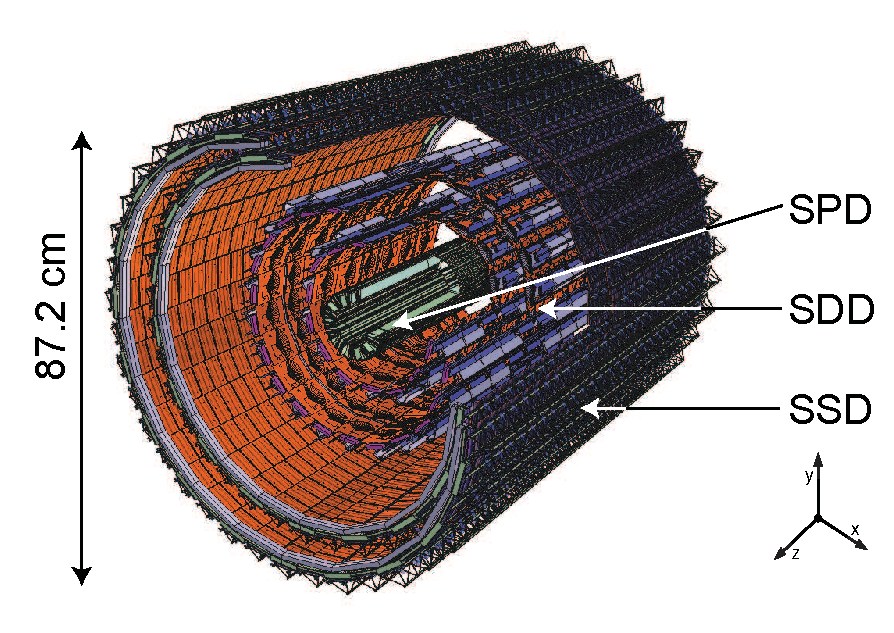
\includegraphics[width=0.75\textwidth]{Figs/Chapter3/its-rf-2-26925.eps}
}
\end{center}
\subfigure[]
{
	\includegraphics[width=0.31\textwidth]{Figs/Chapter3/ALICE-3D-Run1+2-ITS+V0-Inlay-v0-2012-08-02-Highlight-SPD.png}
}
\subfigure[]
{
	\includegraphics[width=0.31\textwidth]{Figs/Chapter3/ALICE-3D-Run1+2-ITS+V0-Inlay-v0-2012-08-02-Highlight-SDD.png}
}
\subfigure[]
{
	\includegraphics[width=0.31\textwidth]{Figs/Chapter3/ALICE-3D-Run1+2-ITS+V0-Inlay-v0-2012-08-02-Highlight-SSD.png}
}
	\caption{Visualisation of the complete structure of the ITS detector (a), as well as a highlight on the SPD(b), SDD(c) and SSD(d) locations in the ALICE apparatus. Figures taken from \cite{alicecollaborationAlignmentALICEInner2017}\cite{maireALICESubdetectorsHighlighted2017}.}
	\label{fig:ITSstructure}
\end{figure}

\begin{table}[t]
    \centering
    \begin{tabular}{b{1.5cm}@{\hspace{0.5cm}} b{1.5cm}@{\hspace{0.25cm}} b{1.5cm}@{\hspace{0.5cm}} b{2cm}@{\hspace{0.5cm}} b{2cm}@{\hspace{0.5cm}} b{1.5cm}@{\hspace{1cm}} b{2cm}@{\hspace{0.cm}}}
    \noalign{\smallskip}\hline\noalign{\smallskip}
	Layer & $r$ (\cm) & $\pm z$ (\cm) & Area ($\m^{2}$) & Active area per module ($\mm^{2}$) & Resolution $r\varphi \times z$ ($\mum^{2}$) & Material budget (\%\Xzero) \\
    \noalign{\smallskip}\hline \noalign{\smallskip}
    1 - SPD & 3.9 & 14.1 & 0.07 & 12.8 $\times$ 69.6 & 12 $\times$ 100 & 1.14 \\
    2 - SPD & 7.6 & 14.1 & 0.14 & 12.8 $\times$ 69.6 & 12 $\times$ 100 & 1.14 \\
    3 - SDD & 15.0 & 22.2 & 0.42 & 72.5 $\times$ 75.3 & 35 $\times$ 25 & 1.13 \\
    4 - SDD & 23.9 & 29.7 & 0.89 & 72.5 $\times$ 75.3 & 35 $\times$ 25 & 1.26 \\
    5 - SSD & 38.0 & 43.1 & 2.20 & 73 $\times$ 40 & 20 $\times$ 820 & 0.83 \\
    6 - SSD & 43.0 & 48.9 & 2.80 & 73 $\times$ 40 & 20 $\times$ 820 & 0.86 \\
    \noalign{\smallskip}\hline\noalign{\smallskip}
    \end{tabular}
    \caption{Details on the six layers of the ITS during the LHC Run-1 and Run-2. \cite{alicecollaborationALICEExperimentCERN2008}\cite{carminatiALICEPhysicsPerformance2004}. The radial distance $r$ are, in fact, average positions. The rightmost column only includes the material budget of the sensor.}\label{tab:ITSspec}
\end{table}

The two innermost layers are positionned at 3.9 and 7.6 \cm from the origin, covering a pseudo-rapidity range of $|\eta| < 2$ and $|\eta| < 1.4$ respectively. At this distance, the track density can reach values up to 80 tracks/$\cm^{2}$. In order to cope with these high track densities, the layers are equipped with SPD employing hybrid\footnote{The term \textit{hybrid} here refers to a type of pixel technology in which the silicon sensor and the readout chip are processed separatedly and connected together via a bump-bonding process. In this way, the detector (silicon sensor) and the electronics (readout chip) can be optimized individually. In LHC experiments, the optimisation is performed such that the detector has a good radiation tolerance and the readout is fast. In return, the assembly tends to be more complex and expensive, the readout chips dissipate a lot of power requiring an efficient cooling system and so more material budget.} silicon pixels. It consists of a bi-dimensional matrix of 256 $\times$ 160 cells of dimension 50 \mum ($r\varphi$) by 425 \mum ($z$). Two matrices are mounted together along the $z$ direction, forming a 141.6 \mm long half-stave. Two of them are attached head to head along the beam direction on a carbon-fibre support with cooling tubes in order to forge a stave. The latter are arranged in ten sectors surrounding the beam pipe, each sector supporting two staves for the inner layer and four for the outer layer. While the high granularity of the SPD provides a spatial resolution of 12 \mum in $r\varphi$ and 100 \mum along $z$, its fast integration time of 100 \nsec -- corresponding to four consecutive bunch-crossings in pp collisions or one in heavy-ions operation -- offers additionnal trigger information.

The SDDs equip the two intermediate layers at an average distance of 15.0 and 23.9 \cm, where the track density rises up to 7 tracks/$\cm^{2}$. Both layers have a pseudo-rapidity acceptance of $|\eta| < 0.9$. The basic module consists in a sensitive area of 70.17 $\times$ 75.26 $\mm^{2}$, split into two drift regions by a central cathode strip at high voltage such that the drift velocity is 8.1 $\mum/\nsec$. At this speed, charges drift to one of the 256 collection anodes (with a 294 \mum pitch) in a maximum time of 4.3 \musec, making it the slowest ITS detector. The SSD modules are mounted on triangular support structure made of carbon-fibre called ladders. The third layer counts 14 ladders with six modules each, and 22 ladders with eight detectors each for the fourth layer. They yield to a spatial precision of 35 \mum in the transverse plane and 25 \mum along the beam axis. 

The two outermost layers are constituted of double sided SSD of 73 $\times$ 40 $\mm^{2}$, where each side has 768 parallel strips (with a pitch of 95 \mum) and corresponds to a side of a p-n junction. The p-side (n-side) of the fifth layer (sixth layer) faces the inside of the ITS. The strips from one side are rotated by a stereo angle of 35 mrad with respect to the other, to reduce the overlapping between the strips and thus the number of ambiguities. The SSD modules are assembled on the same ladder design as those of the intermediate layers: 34 ladders, supporting 22 modules each, are installed on average at 38 \cm from the beam pipe for the inner layer and 38 ladders, holding 25 modules each, at 43 \cm for the outer layer. Both covers a pseudo-rapidity region of $|\eta| < 0.9$. The SSDs layers provide a spatial resolution of the track position of 20 \mum in the $r\varphi$ direction and 820 \mum along $z$, which is essential for the track matching from the Time Projection Chamber to the ITS. Similarly to the SDD layers, its analogue readout allows for the measurement of the charge deposited by the passage of a charged particle, and hence opens the door for PID of low-momentum particles.

Because of the sensitivity of the SDD layers to temperature changes, two thermal shields surround them in order to avoid any radiation of heat.


\subsubsection{Time Projection Chamber}
\label{subsubsec:TPC}

\begin{figure}[t]
\subfigure[]
{
	\includegraphics[width=0.62\textwidth]{Figs/Chapter3/1-s2.0-S0168900210008910-gr2_lrg.jpg}
	\label{fig:TPCFieldCage}
}
\subfigure[]
{
	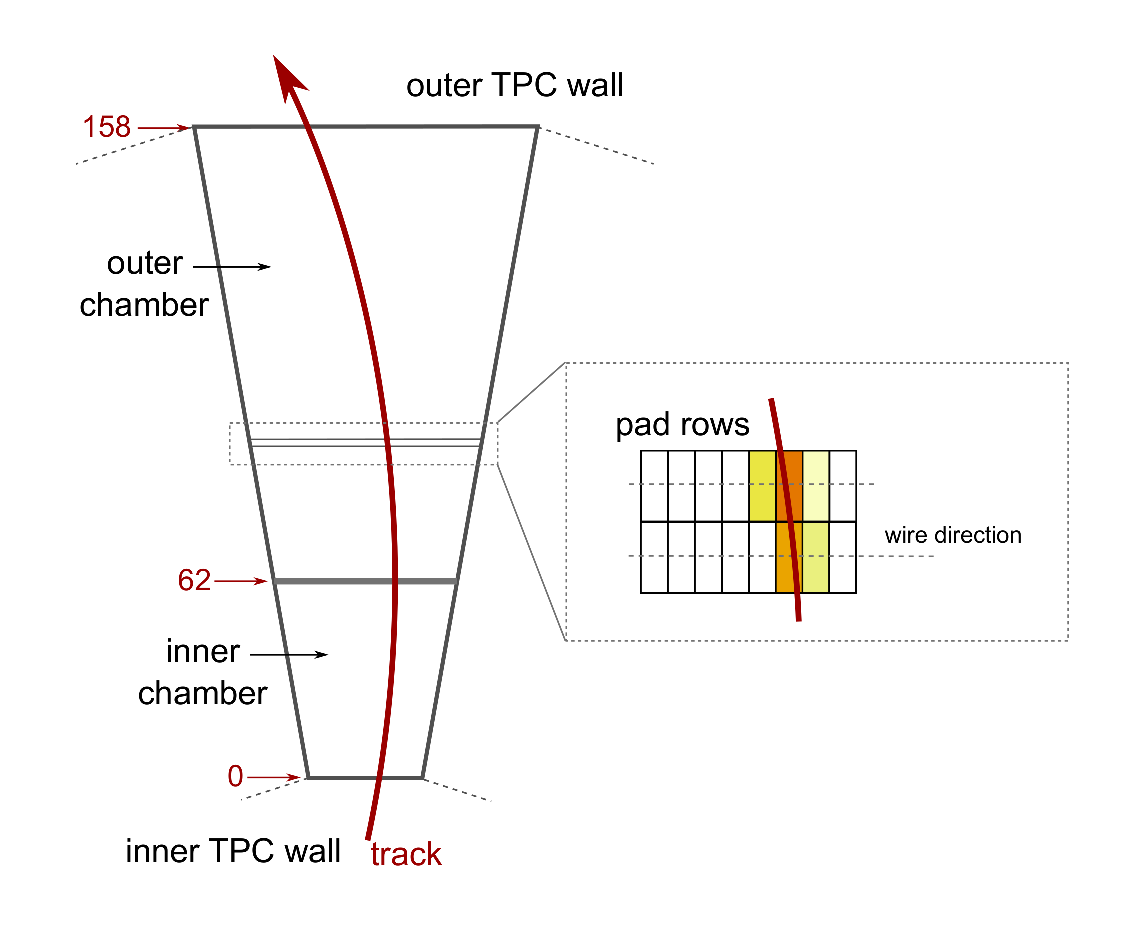
\includegraphics[width=0.50\textwidth]{Figs/Chapter3/Schema-TPC-SecteurEtPadRow.eps}
	\label{fig:TPCSector}
}
	\caption{(Left panel) Scheme of the TPC field cage, taken from \cite{almeALICETPCLarge2010}. (Right panel) Passage of a charged particle through a sector of the TPC. Figure taken from \cite{maireALICETPCSectors2011}.}
	\label{fig:TPCDetector}
\end{figure}

The Time Projection Chamber (TPC) is main tracking device of the ALICE experiment. It is responsible for measuring the momentum of charged particle above 150 \mmom, as well as providing particle identification and vertex determination. The TPC design is shown in \fig\ref{fig:TPCFieldCage}. It consists in a cylindrical gaseous detector, encercling the ITS, with an inner radius of about 85 \cm, an outer radius of 250 \cm and an overall length of 500 \cm along the beam axis. The acceptance of the TPC covers pseudo-rapidities from $|\eta| < 0.9$ (for tracks traversing radially the entire ALICE detector) up to $|\eta| = 1.5$ and the full azimuth (except for the dead zones between sectors). Although this detector occupies a large volume, its material budget remains low (about 3.5\% \Xzero).

The detection volume corresponds to a field cage filled with gas and separated in two equal parts, along the beam axis, by a central electrode at -100 kV. At this high voltage, this central membrane generates an axial electrostatic field of 400 V/\cm. When a charged particle traverses the 88 $\m^{3}$ active volume, it creates electron-hole pairs along its path by ionisation of the gas. The electrostatic field forces the electrons to drift from the central electrode to the end plates, where they are collected, in a maximum time of 92 \musec at a speed of 2.7 \cm/\musec (depending on the gas composition).

Each end plate is segmented into 18 trapezoidal sectors (as represented in \fig\ref{fig:TPCSector}), being themselves instrumented with two multi-wire proportionnal chambers (MWPC) with cathode pad readout: one stretches from $R= 84.8$ \cm to 132 \cm (inner chamber), the other ranges from 134.6 \cm to 246.6 \cm (outer chamber). This is motivated by the variation of the track density with the radius, that requires MWPCs with different wire geometry and pad sizes (granularities). Together, the two chambers count a total of 159 readout pad rows: 63 of 4 $\times$ 7.5 $\mm^{2}$ for the inner chamber, 64 of 6 $\times$ 10 $\mm^{2}$ and 32 of 6 $\times$ 15 $\mm^{2}$ for the outer chamber. They measure the deposited charge, as well as the radial position and the drift time. The longitudinal coordinate is inferred from the latter, provided that the drift speed is uniform over the whole volume\footnote{The longitudinal position is thus given by the product of the drift velocity and the drift time.}. In fact, the gas composition has been optimised for high and stable drift velocity, as well as low diffusion and small radiation length. At the start of the LHC Run-2, a mixture of Ne/CO$_{2}$/N$_{2}$ (90/10/5\%) was employed until 2017. It was later changed for Ar/CO$_{2}$ (90/10\%) as the latter reduces the space-charge distortion [ref?].

\begin{figure}[t]
	\centering
	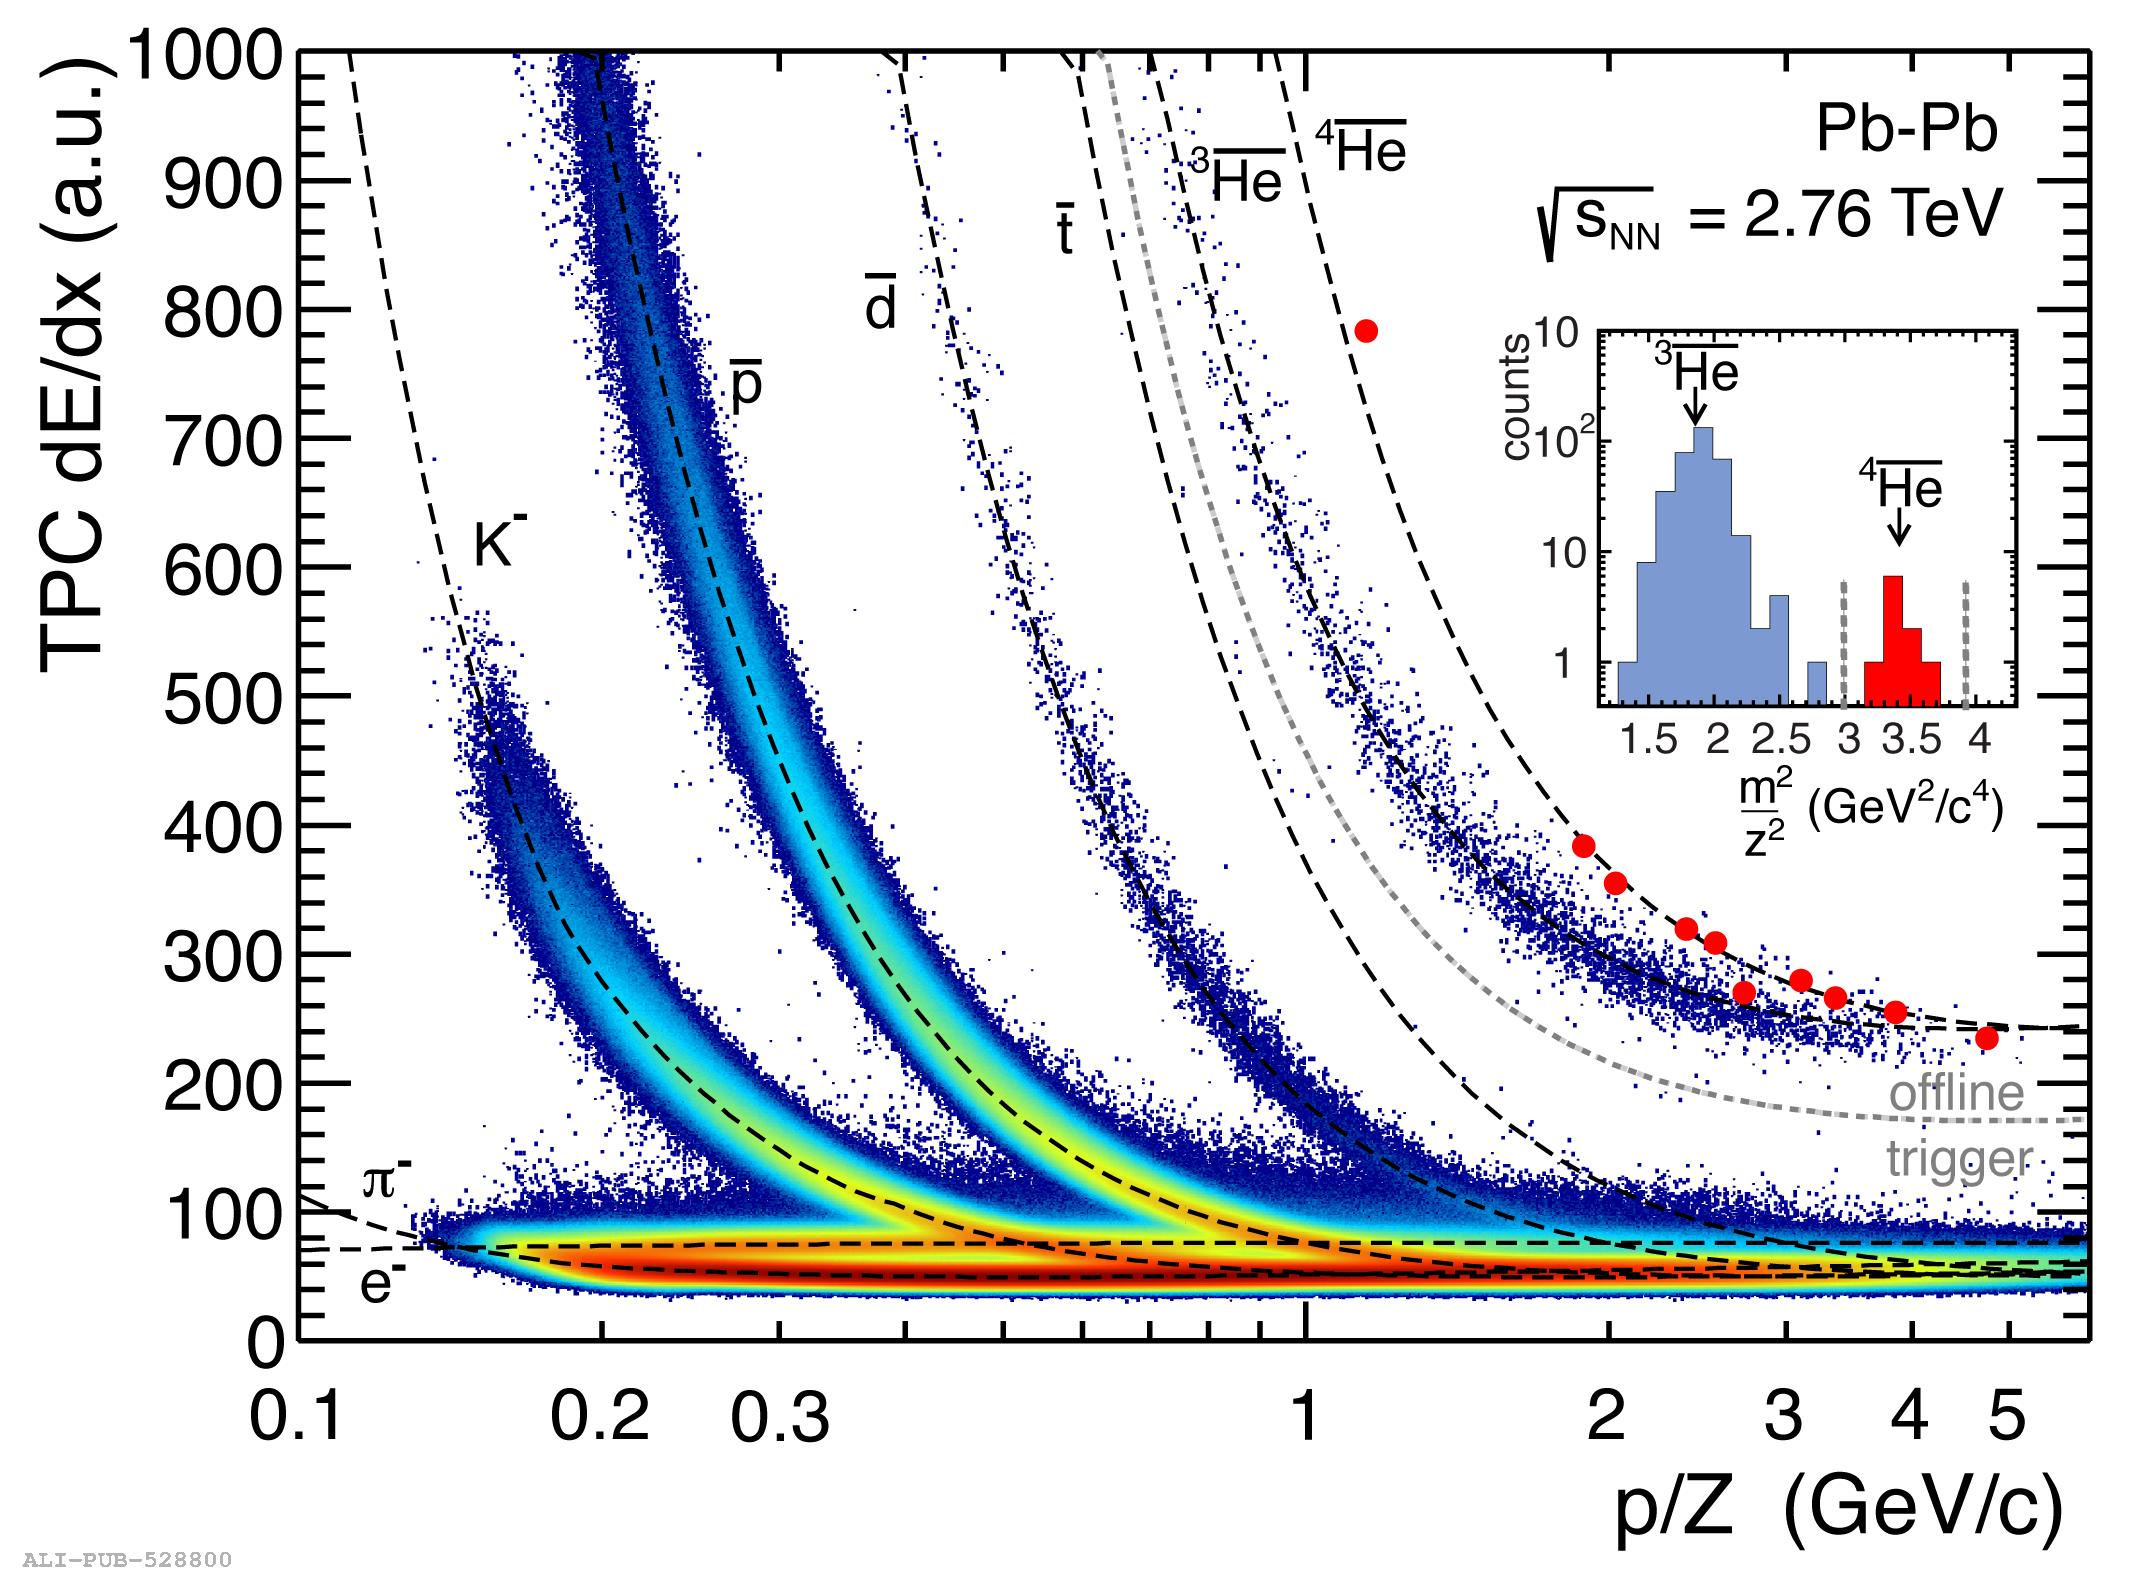
\includegraphics[width=0.8\textwidth]{Figs/Chapter3/dEdx_PbPb_2011_withAlphaInlet_NoLogo.eps}
	\caption{Energy deposition of various charged particles (electron, pion, kaon, anti-proton, anti-deuteron, anti-tritium, and two anti-helium isotopes) in the ALICE TPC in arbitrary units as a function of the magnetic rigidity (momentum over charge number). The dashed lines correspond to the theoretical expectations for each particle species. Figure taken from \cite{alicecollaborationALICEExperimentJourney2022}.}
	\label{fig:TPCdEdx}
\end{figure}

The spatial resolution varies from 1100 to 800 \mum in the transverse plane, and 1250 to 1100 \mum along the beam axis. Although the TPC can not compete with the level of precision of the ITS, it stands as the main tracking detector in ALICE thanks to its almost continuous sampling of the particle trajectory over large distances.

Moreover, the pad rows provides an analogue readout of the charge deposition, that is used to measure the energy loss of charged particles per unit of length (\dEdx) with a resolution ($\sigma_{\rm TPC}$) ranging from 5.5\% in pp events to 6.5\% in the most central Pb-Pb collisions. As the energy deposition is stochastic phenomenon, only the moments of its underlying distribution can be predicted. For instance, the Bethe-Bloch formula describes the mean \dEdx:
\begin{equation}
\begin{split}
\langle -\frac{dE}{dx} \rangle &= K z^{2} \frac{Z}{A} \frac{1}{\beta^{2}} \left[ \frac{1}{2} \ln \frac{2 m_{e} c^{2} \beta^{2} \gamma^{2} T_{\rm max}}{I} - \beta^{2} - \frac{\delta \left( \beta \gamma \right)}{2} \right],\\
\beta \gamma &= \frac{p}{M c}
\end{split}
\label{eq:BetheBloch}
\end{equation}
with 
\begin{itemize}
\item[$\bullet$] $Z$, the atomic number of the absorber (the TPC gas in this case),
\item[$\bullet$] $A$, the atomic mass of the absorber (g.mol$^{-1}$),
\item[$\bullet$] $m_{e}$, the electron mass,
\item[$\bullet$] $z$, charge number of the incident ionising particle,
\item[$\bullet$] $M$, mass of the incident ionising particle,
\item[$\bullet$] $p$, momentum of the incident ionising particle,
\item[$\bullet$] $\beta$, velocity of the incident ionising particle in units of $c$,
\item[$\bullet$] $\gamma$, Lorentz factor of the incident ionising particle,
\item[$\bullet$] $I$, mean excitation energy of the absorber,
\item[$\bullet$] $\delta \left( \beta \gamma \right)$, density effect correction due to the polarisation of the absorber,
\item[$\bullet$] $T_{\rm max} = \frac{2 m_{e} c^{2} \beta^{2} \gamma^{2}}{1 + 2 \gamma m_{e}/M + \left( m_{e}/M \right)^{2} }$, the maximum energy transfer to an electron in a single collision, 
\item[$\bullet$] $K$, a constant.
\end{itemize}

As a matter of fact, the energy deposition follows a Landau distribution. Its broad tail on the high-energy-loss side leads the mean energy loss to be considerably greater than the most probable value. It turns out that the most probable energy loss is much easier to evaluate than the mean, requiring large samples to converge. Thereby, the Landau distribution is usually truncated only to keep the 50 to 70\% smallest values, and by so doing, the truncated mean coincides with the most probable energy loss \cite{particledatagroupReviewParticlePhysics2022}.\\


\Fig\ref{fig:TPCdEdx} shows clearly the characteristic \dEdx bands associated to \electron, \rmPi, \proton, \rmDeuton, \rmTriton, \rmHeThree and \rmHeFour. The measurements distribute around dashed lines, that correspond to the expected mean value given by the Bethe-Bloch formula (\eq\ref{eq:BetheBloch}). By comparing the measured value to the expected energy loss for various particle species, the nature of the incident particle can be determined. The PID estimator
\begin{equation}
n_{\sigma} = \frac{ \langle \dEdx \rangle_{\rm meas} - \langle \dEdx \rangle_{\rm exp, i}}{\sigma_{\rm TPC}}
\end{equation}
gives the distance between measured \dEdx and the expected one under the particle mass hypothesis $m_{\rm i}$ (i $=$ \electron, \rmPi, \proton, \rmDeuton, \rmTriton, \rmHeThree, \rmHeFour), in units of relative resolution $\sigma_{\rm TPC}$. So, the TPC can distinguish a pion/electron from a kaon with a separation power better than 3$\sigma$ below $\sim$ 300 \mmom, and a kaon from a proton up to 1 \gmom.

\begin{figure}[b]
\centering
\subfigure[]
{
	\includegraphics[width=0.6\textwidth]{Figs/Chapter3/ALICE-3D-Run1+2-ITS+V0-Inlay-v0-2012-08-02-Highlight-VZERO.png}
	\label{fig:VZEROinALICE}
}	
\subfigure[]
{
	\includegraphics[width=0.8\textwidth]{Figs/Chapter3/Fig1-4206.png}
	\label{fig:VZEROarrays}
}
	\caption{(Top panel) View of the VZERO scintillator arrays inside the ALICE apparatus: VZERO-A on the left, and VZERO-C on the right. (Bottom panel) Sketches of the VZERO-A (left) and VZERO-C (right) with their segmentation. The dashed lines delimit segments connected to the same photomultiplier tube. Figures taken from \cite{alicecollaborationALICEExperimentJourney2022}\cite{alicecollaborationPerformanceALICEVZERO2013}.}
	\label{fig:VZEROdetector}
\end{figure}


\subsubsection{VZERO}
\label{subsubsec:VZERO}

The VZERO system consists in two scintillator arrays, VZERO-A and VZERO-C, covering the pseudo-rapidity ranges $2.8 < \eta < 5.1$ and $-3.7 < \eta < -1.7$ respectively (\fig\ref{fig:VZEROinALICE}). It plays a crucial role in the data taking of ALICE as it provides minimum-bias triggers for the experiment, measures the charged particle multiplicity and centrality, and participates in the beam luminosity determination.


Each of array is segmented in four rings, themselves being divided in eight sections of 45 wide made of plastic scintillators, as sketched in the \fig\ref{fig:VZEROarrays}. Because of the integration constraints (mainly coming from the muon absorber), two arrays needed to be designed. The 2.5 \cm thick VZERO-A sits at 329 \cm from the nominal vertex ($z = 0$). Since the VZERO-C stands in front of the muon absorber, the scintillator thickness reduces to 2 \cm and its rings are positionned between -86 and -88 \cm along the beam axis. 

\begin{figure}[h]
	\centering
	\includegraphics[width=0.8\textwidth]{Figs/Chapter3/Fig6_2-4228.png}
	\caption{Time of flight of the particles detected in the VZERO-C versus VZERO-A. Figure taken from \cite{alicecollaborationPerformanceALICEVZERO2013}.}
	\label{fig:VZERObeamgas}
\end{figure}

The passage of a charged particle in the scintillator generates light, that is guided to photomultiplier tubes via 1 \mm in diameter Wave-Length Shifting and optical fibers. For each of the 32 elementary cells, the photomultiplier tube outputs two analogue signals. The first measures the integrated charge, the second -- amplified by a factor 10 -- determines the pulse/arrival time relative to the LHC bunch clock with a resolution better than 1 \nsec. Each signal gives rise to a specific type of trigger algorithm. 

Based on the coincidence between the time signals from the arrays, beam-induced background events\footnote{They typically correspond to beam-gas collisions, that is a collision between a bunch from the beam and a residual atom in the beam pipe} can be rejected. \Fig\ref{fig:VZERObeamgas} shows an example of such rejection. A particle coming from the interaction point takes about 11 \nsec and 3 \nsec to reach the VZERO-A and the VZERO-C respectively. If the time of flight of the particles detected in the two scintillator arrays matches these values --- as it is the case in the top right corner of \fig\ref{fig:VZERObeamgas} ---, this would indicate that a beam-beam collision occured. However, the signals arriving in coincidence at -12 \nsec (VZERO-A) and 3 \nsec (VZERO-C), and 11 \nsec (VZERO-A) and -3 \nsec (VZERO-C) are not the signatures of a beam-beam event. They correspond to beam-gas collisions coming from the A-side and C-side respectively. This is the first type of trigger algorithm.

The energy deposited in the scintillators provides a measurement of the charged particle multiplicity. Based on a simulation of VZERO detectors, the total charge collected can be related to the number of primary charged particles. \Fig\ref{fig:VZEROcentrality} shows the relation between these two quantities. The second type of trigger algorithm consists in dividing the distribution of the V0 amplitudes in different multiplicity/centrality\footnote{In heavy-ion collisions, as in \fig\ref{fig:VZEROcentrality}, the impact parameter -- and, \textit{a fortiori}, its percentage value, the centrality -- can not be measured directly. However, since the centrality and the charged particle multiplicity in the event are correlated (confirmed by Glauber fit, that gives access to the centrality), the different intervals in multiplicity are refered as \textit{centrality classes}.} classes from the 5\%-highest multiplicity to the 10\%-lowest multiplicity events, as represented in shaded areas. 

\begin{figure}[h]
	\centering
	\includegraphics[width=0.8\textwidth]{Figs/Chapter3/Fig8-4236.png}
	\caption{Total yield as a function of the signal amplitudes of the two VZERO arrays in Pb-Pb collisions at \sqrtSnn = 2.76 \tev, fitted with a Glauber model in red. The shaded areas correspond to different centrality classes. Figure taken from \cite{alicecollaborationPerformanceALICEVZERO2013}.}
	\label{fig:VZEROcentrality}
\end{figure}

\subsubsection{Time-Of-Flight detector}
\label{subsubsec:TOF}

The Time-Of-Flight (TOF) detector is a large cylindrical array with an inner radius of 370 \cm and an outer one of 399 \cm. It covers the central pseudo-rapidity region, that is $|\eta| < 0.9$, and the full azimuth. While the separation power of TPC only goes up to 1 \gmom, the TOF detector aims at providing particle identification at intermediate momentum from 0.2 to 2.5 \gmom.  To instrument this large volume (17.5 $\m^{3}$), a gaseous detector is employed, as its manufacture remains rather simple and thus inexpensive. The best solution, with respect to the design considerations of the experiment, is the Multi-gap Resistive-Plate Chamber (MRPC) \cite{akindinovMultigapResistivePlate2000}. 

The basic constituent of the TOF system is a pair of MRPC strips, 122 \cm in length and 12 \cm in width, stacked together with an active area of 120 $\times$ 7.4 $\cm^{2}$. As shown in \fig\ref{fig:TOFMRPC}, it consists in two cathodes and a central anode placed in a gas volume and spaced by five 0.4 \mm thin glass plates (with a 250 \mum gap) for each strip. The full volume is filled with a gas mixture composed of C$_{2}$H$_{2}$F$_{4}$(90\%), C$_{4}$H$_{10}$(5\%), SF$_{6}$(5\%), as it shows no ageing effects and  has a rate capability much higher than the expected one in ALICE \cite{akindinovStudyGasMixtures2004}.

\begin{figure}[t]
\hspace*{-1.5cm}
\subfigure[]
{
	\includegraphics[width=0.5\textwidth]{Figs/Chapter3/TOFMRPC.png}
	\label{fig:TOFMRPC}
}
\subfigure[]
{
	\includegraphics[width=0.75\textwidth]{Figs/Chapter3/TOFSuperModule.png}
	\label{fig:TOFStructure}
}	
	\caption{(Left panel) Drawing of the cross section of a 10-gap double-stack MRPC. (Right panel) Schematic view of the TOF barrel with one supermodule, consisting of five modules. Figure taken from \cite{alicecollaborationALICEExperimentCERN2008}.}
	\label{fig:TOFPID}
\end{figure}

To cover the full cylinder along the beam direction and minimise the cumulative dead areas from the innermost to outermost detectors in ALICE, five modules of different lengths are combined. The central element utilizes 117 \cm long module, the intermediate ones 137 \cm, the external ones 177 \cm made of 15 MRPC strips for the central module and 19 for the others. Altogether, they form a supermodule of total length 930 \cm with an overall active region of 741 $\times$ 7.4 $\cm^{2}$, as shown on \fig\ref{fig:TOFStructure}. Each of the 18 azimuthal sectors of the TOF system has a supermodule.

When a charged particle traverses the active volume, it ionises the gas along its path and produces electrons that drift to one of the cathodes. The key aspect of the MRPC resides in the high voltage of the anode (-13 kV), which delivers a high and uniform electrostatic field. The latter is sufficiently strong to start an avalanche process\footnote{Let us consider a medium containing free electrons and in which a strong electrostatic field exists. If the latter is strong enough, it accelerates the electrons such that they will collide with other atoms in the medium, thereby ionising them and releasing additionnal electrons. These ones also get accelerated and collide with other atoms, releasing more electrons, and so on. This chain reaction is called an avalanche process.}, and thereby to give rise to a detectable signal. The avalanche stops when it reaches a glass plate, but the produced electrons continue to drift -- and to create avalanches in the gaseous medium along the way -- until they are collected by the 48 cathode pad readouts of 3.5 $\times$ 2.5 $\cm^{2}$ from each strip. \\

Their output signals carry the information of the deposited charge via the Time-Over-Threshold and the hit time -- with an intrinsic resolution of 56 \psec during the LHC Run-2 -- relative to the collision time, $t_{\rm ev}$. Due to the finite size of the bunches that interact, the latter has to be measured on an event-by-event basis. To that end, different options are available.

The most precise measurement of the collision time is provided by the T0 detector. It consists in two arrays, each made of twelve Cerenkov counters, placed at 375 (T0-A) and -72.7 \cm (T0-C) from the nominal vertex. They respectively cover the pseudo-rapidity range $4.61 < \eta < 4.92 $ and $-3.28 < \eta < -2.97$. Each counter is a quartz radiator of 20 \mm in diameter and 20 \mm thick, connected optically to a PMT. The readout electronics is quite similar to the one used for the TOF detector, with a dead time below 25 \nsec. The T0 system gives two time measurements, $t_{\rm T0-A}$ and $t_{\rm T0-C}$, one for each array. When both values are available, the average is taken as the start time of the event, $t_{\rm ev}^{\rm T0} = \left( t_{\rm T0-A} + t_{\rm T0-C} \right)/2$, with a resolution of 50 and 25 \psec in pp and Pb-Pb collisions. If only one of the two counters produces a signal, the collision time is given by either the $t_{\rm T0-A}$ or $t_{\rm T0-C}$ taking into account the longitudinal position of the primary vertex (provided by the ITS). Consequently, the resolution deteriorates to 100 and 60 \psec in pp collisions for the T0-A and -C respectively, and 50 and 30 \psec in heavy-ion collisions. Due to its limited acceptance, the triggering efficiency of the detector in coincidence is about 48\%, and reaches 60\% and 67\% for the T0-A and -C individually in pp collisions\footnote{The triggering efficiency is close to 100\% in heavy-ion collisions, due to the high multiplicities.}.

The TOF system itself can also determine $t_{\rm ev}$. Based on a sample of particles matching a hit in the detector, a $\chi^{2}$-minimisation procedure is performed in order to extract the set of mass hypotheses that minimises their combined time-of-flights. From this set derives the event collision time, denoted $t_{\rm ev}^{\rm TOF}$. By construction, this procedure only applies for a minimum number of two tracks, and the resolution improves with the track multiplicity (scaling as $\sim 1 / \sqrt{n_{\rm tracks}}$). It allows to reach time resolution from 80 \psec for the low multiplicity events to 20 \psec for the high multiplicity events, with efficiencies ranging from 20\% to 100\% respectively.

Considering the above efficiencies, the collision start time can be obtained from the T0 or TOF measurement ($t_{\rm ev}^{\rm T0}$ or $t_{\rm ev}^{\rm TOF}$) or their combination, if both are available. In the latter case, the final $t_{\rm ev}$ corresponds to their weighted average, with the inverse of their resolution squared as weighting factors. If none of the preceding procedures is usable, the event time is set on the LHC clock\footnote{In fact, it is set on zero as, after alignement and calibration of the TOF detector, the LHC clock phase has been shifted to coincide with the nominal starting time.} which has a resolution of 200 \psec \cite{alicecollaborationDeterminationEventCollision2017}.\\



Hence, the difference between the arrival time $t_{\rm TOF}$ and the moment of the collision $t_{\rm ev}$ gives the \textit{measured time-of-flight} of the charged particle from the primary vertex to the TOF detector. Knowing the latter as well as the the distance travelled, the velocity of the particle -- or rather the ratio of the velocity to the speed of light, $\beta = v /c$ -- can be evaluated. The \fig\ref{fig:TOFPID} shows the distribution of $\beta$ of charged particles measured by the TOF detector as a function of their momentum in Pb-Pb events at \sqrtSnn = 5.02 \tev. A clear separation of the electron, pion, kaon, proton and deuteron bands is visible. This stems from the relation between the particle mass $m$, its momentum $p$ and its velocity $\beta$: 
\begin{align}
m = \frac{p}{\beta \gamma} = p \ \sqrt{ \frac{1}{\beta^{2}} - 1 }& \qquad \textrm{with} \quad \beta = \frac{v}{c} = \frac{L}{c t_{\rm exp}},\\
\Rightarrow t_{\textrm{exp}} &= L \ \frac{\sqrt{p^{2} + m^{2}}}{c p}.
\label{eq:tTOF}
\end{align}

\begin{figure}[t]
	\centering
	\includegraphics[width=0.8\textwidth]{Figs/Chapter3/TOFBetawoMismatchEtaCut_PbPb.eps}
	\caption{Velocity ($\beta = v /c$) of electrons, pions, kaons, protons and deuterons as a function of their momentum (provided by the TPC), measured by the TOF detector, in Pb-Pb collisions at \sqrtSnn = 5.02 \tev. Figure taken from \cite{alicecollaborationALICEExperimentJourney2022}.}
	\label{fig:TOFPID}
\end{figure}

In \eq\ref{eq:tTOF}, $t_{\textrm{exp}}$ corresponds to the \textit{expected time-of-flight}, \ie the time it would take for a particle of mass $m$, with a momentum $p$, to go from the interaction point to the TOF detector following a path of length $L$. To this quantity is attached an uncertainty coming from the track reconstruction, as it will be detailed in \Sec\ref{subsec:EventReco}. By comparing the measured time-of-flight $t_{\rm TOF}$ and the expected one $t_{\rm exp, i}$ for different mass hypothesis $m_{\rm i}$ (i $=$ \electron, \muon, \rmPi, \rmKaon, \proton, \rmDeuton, \rmHeThree, \rmHeFour), particle identification can be performed. The PID estimator $n_{\sigma}$ is constructed in the following way:

\begin{equation}
n_{\sigma} = \frac{t_{\rm TOF} - t_{\rm ev} - t_{\rm exp, i} }{\sigma_{\rm PID, i}}, \qquad \text{with} \quad \sigma_{\rm PID, i}^{2} = \sigma_{t_{\rm TOF}}^{2} + \sigma_{t_{\rm ev}}^{2} + \sigma_{t_{\rm exp, i}}^{2}.
\end{equation}

Therefore, the TOF detector is capable of identifying charged particles in the intermediate momentum range, with a separation power better than 3$\sigma$ between pions and kaons below 2.5 \gmom, and up to 4 \gmom between kaons and protons.

\subsection{Trigger system and data acquisition}

As opposed to its LHC Run-3 version, ALICE only recorded triggered data in the Run-1 and -2, \ie events are selected and stored based on a variety of different features. The Central Trigger Processor (CTP) is in charge of optimising the trigger system in order to make the best use of i) the various detector components, that are busy for different period of time ($\sim$88 \musec for the TPC versus the T0 with $<$25 \nsec) when a valid trigger signal is received, and ii) the different running modes (pp, pPb, PbPb with specific interaction rates).\\

The latter is achieved by ensuring that the data collection is not ruined by the pile-up. Here, we refer primarily to event pile-up between different bunch crossings, that is treated differently depending on the expected multiplicity and luminosity. The one occuring between two central or semi-central heavy-ion collisions must be avoided as the density of tracks is so high that they become unreconstructable. However, the pile-up level between a (semi-)central and up to two peripheral Pb-Pb collisions is tolerable in some detectors -- such as the TPC -- and not in others -- the ITS for example. The same applies for pp collisions where pile-up is unavoidable but tracks are reconstructable due to much lower track densities than in Pb-Pb. To that end, a \textit{past-future} protection has been implemented, which basically verifies that the level of pile-up in the sensitive time windows of each detector\footnote{For instance, the past-future protection circuit checks on the TPC that the pile-up occuring between -88 \musec (past) and +88 \musec (future) relative to the collision time stays managable. The same logic applies to the rest of the ALICE devices. In fact, three categories of detectors can be drawn: the ones that can provide a signal at each bunch crossing and thus do not not need a protection, the others requiring the application of the past-future condition under 10 \musec, and the TPC demanding a protection under 88 \musec.} remains tolerable as defined in the above requirements.\\

To ensure efficient data taking, the ALICE detector is not entirely readout for every event. Instead, it is divided into groups of sub-systems named detector \textit{clusters}. For instance, the data from the forward muon arm do not need the TPC to be exploitable, only the trigger detectors (in particular the V0 and SPD for determining the centrality/multiplicity class and primary vertex location) are required. By grouping these detectors into the same cluster, they can be read out separately from the other devices. Consequently, there are three detector clusters comprising the full detector, only the central detectors, and the forward muon detectors (with the trigger detectors) respectively.

In addition, the hardware trigger system divides into three levels -- dubbed L0, L1 and L2 -- with different latencies \cite{bloodworthALICECentralTrigger2000}\cite{alicecollaborationTriggerDataAcquisition}. At each LHC clock cycle (that is every 25 \nsec in pp and 100 \nsec in heavy-ion mode), the CTP checks for the inputs from detectors with fast trigger capabilities (essentially the T0, V0, SPD and TOF) up to 800 \nsec after the collision (time needed for the SPD to transmit its trigger signal to the CTP). When the inputs coincide with the requirements of one (or more) \textit{trigger class}\footnote{This is the set of detector signals that defines a trigger selection. The ALICE experiment counts 50 trigger classes \cite{alicecollaborationALICEExperimentCERN2008}.}, the trigger system issues a Level 0 (L0) decision in less than 100 \nsec, that reaches the detectors 1.2 \musec after the interaction. Upon reception of the L0 signal, detectors move into a busy-state in which they stop taking new data until they have been fully read out. Since all the detector inputs can not be transmitted under 800 \nsec, the CTP collects all the signals that can be delivered under 6.1 \musec, checks the conditions for all trigger classes and -- in the absence of a veto from the past-future protection circuit -- generates a Level 1 (L1) trigger arriving at the detectors 6.5 \musec after the collision. Together, the L0 and L1 signals represent the fast response of the trigger system. The last signals arrives 87.6 \musec after the collision, due to the drift period of the TPC. A level 2 (L2) trigger decision is sent with a latency of 100 \nsec and reaches the detectors at 88 \musec, to finally conclude on whether the event is accepted or rejected. At this stage, a rejection most often comes from the excessive pile-up.\\

Among the different trigger classes, two configurations play an important role in ALICE and in the present work: the minimum-bias (MB) and the high-multiplicity (HM) classes. As its name suggests, the former refers to the least biasing conditions for the data acquisition in ALICE over the full multiplicity distribution. Its requirements have evolved over the years. Because of the low interaction rate in pp in 2009 and 2010 data takings, the minimum-bias trigger selections were kept loose: it required a hit in either VZERO counters or in one of the two SPD layers (MB$_{\rm OR}$). In this way, the collected event would have at least one charged particle in eight units of pseudo-rapidity. As the luminosity and the amount of beam-gas background increase, the conditions were tightened up and the high selection efficiency MB trigger is traded off for a high purity one. Hence, to be recorded, an event necessitates a coincidence between the VZERO detectors (MB$_{\rm AND}$). This is equivalent of asking for, at least, one charged particle in the A- and C-side, separated by 4.5 units of pseudo-rapidity\footnote{In fact, there exists still a few variants of the minimum-bias trigger such as at least a one hit in the SPD, or one hit in either VZERO scintillator arrays, or even both simultaneously.} \cite{alicecollaborationChargedparticleMultiplicityMeasurement2010}\cite{alicecollaborationALICETriggerCoordination2020}. 

The HM trigger corresponds to 0.1\% highest multiplicity events from the MB sample; it has been implemented in order to study efficiently rare signals, and most particularly in small systems. Throughout the LHC Run-1, it was based the number of hits in the outer layer of the SPD for the multiplicity estimation. The threshold was typically set between 80 to 100 hits which represent about 60 to 80 pairs of matching clusters between the two SPD layers, also refered as SPD tracklets (HM$_{\rm SPD}$) \cite{alicecollaborationALICETriggerCoordination2020}. However, in the Run-2, the default HM trigger configuration changes and the threshold now relies on the signal amplitude of the VZERO counters, that correlates with the event multiplicity (HM$_{\rm VZERO}$). 

As a side note, the trigger system operates in two modes: the default option, called "CENT", corresponds to the one where events are recorded with the informations of the SDD; if this detector is busy at the reception of the L0 signal, the "FAST" configuration allows to record the event without reading out the SSD. Because it is the slowest ITS detector (4.3 \musec) compared to the others (300 \nsec for the SPD and 1.4 to 2.2 \musec for the SSD), the SDD limits significantly the triggering rate. By combining these two trigger configurations (CENT and FAST), one can double the amount of data available but at the price of a lower track reconstruction efficiency (\ref{subsec:TrackReco}).\\

The reception of a successful L2 trigger signal initiates the detectors readout. Each one produces \textit{event fragments} that are transmitted to Data AcQuisition (DAQ) readout receiver cards, being themselves linked to Local Data Concentrators (LDCs). The latter gathers the event fragments from its associated cards and assembles them into sub-events. In parallel, a copy of the readout data is transfered to the High-Level Trigger (HLT) farm computer, that performs an online processing in order to filter out interesting physics events with more sophisticated and precise selections (jet identification, sharp \pT cut, etc) than the lower layer triggers (L0, L1, L2). It can also reduce the output size by selecting relevant parts of the event. The triggered event or the regions of interests are compressed, transfered back to the LDCs. The DAQ system treats the output of HLT system as the one of any other sub-detector.

A single machine of the Global Data Collector (GDC) farm\footnote{The Event-Destination Manager (EDM) supervises the distribution of LDC's sub-events from the same event to single GDC machines, and balances the data stream in order to avoid event loss by overloading the GDC farm (the so-called back-pressure). The latter point is critical for the reconstruction of rare events, as more frequent events take up most of the GDC load. Hence, the EDM monitors their GDC occupancy and, in case it is too high, they are blocked in favour of the rare events. With the past-future protections, these are the causes of a rejection at the L2 trigger stage.} receives the sub-events from sub-detectors' LDCs --- including the ones from the HLT computers -- and proceeds to the event reconstruction. The Transient Data Storage archives the output data over the storage network before their final recording into the Permanent Data Storage.


\subsection{The event reconstruction}
\label{subsec:EventReco}

The event reconstruction starts at the DAQ-LDC level, where the digitised signals of each detector -- likely generated by the same particle -- are grouped into a \textit{cluster}, based on their space and/or time proximities. Its centre of gravity is often taken as an estimate for the crossing point of a particle in the sensitive volume of the detector.

\subsubsection{Preliminary determination of the primary vertex}

From these clusters in the two innermost layers of the ITS, a preliminary estimation of the primary vertex position is realised \cite{caffarridavideCharmSuppressionPbPb2012}. The pairing of SPD clusters between the inner and outer layers (within an azimuthal window of $\Delta \phi = 0.01$ rad) allows to form tiny track segments\footnote{The track curling being supposedly small between the radii of the two SPD layers (3.9 and 7.6 \cm), it can be approximated as a straight line, in particular in the case of high-momentum particles \cite{carminatiALICEPhysicsPerformance2004}.} called \textit{tracklets}. The space point towards which the maximum number of tracklets converges gives a first estimate of the primary vertex location. 

Concretely, the reconstruction algorithm attempts to minimise the quantity
\begin{equation}
D^{2} = \sum_{i}^{N} \left( \frac{x_{i} - x_{0}}{\sigma_{xi}} \right)^{2} + \left( \frac{y_{i} - y_{0}}{\sigma_{yi}} \right)^{2} + \left( \frac{z_{i} - z_{0}}{\sigma_{zi}} \right)^{2},
\label{eq:SPDVertexer}
\end{equation}
with $N$ the number of considered tracklets, and each term of the sum corresponds to weighted distance along $x$, $y$ or $z$ between the tracklet $i$ ($x_{i}, y_{i}, z_{i}$)\footnote{Here, this is the tracklet's position at the point of minimum distance with respect to the primary vertex. At the start of the minimisation procedure, the initial location of the vertex is taken as the mean position of the intersection point of all selected tracklets \cite{carminatiALICEPhysicsPerformance2004}.} and the interaction point ($x_{0}, y_{0}, z_{0}$). The minimisation procedure is repeated several times; at each iteration, the tracklets contributing to a previously found vertex are discarded from the sample. Hence, by construction, the first reconstructed vertex takes up the majority of the contributing tracklets and is designated as the primary one. Since the spatial resolution scales as $1/\sqrt{N_{\rm tracklets}}$, the latter also turns out to be the most accurate. 

In cases where no convergence point is found (as it happens in low-multiplicity events), the algorithm searches for a vertex along the beam axis, with the constraint that it coincides with the beam position in the transverse plane. It is calculated as the weighted mean of the intersection points with the beam axis over all the tracklet candidates.

If no pair of clusters can be formed in the SPD, the primary vertex and thus the event are not reconstructed.

\subsubsection{Track reconstruction}
\label{subsubsec:TrackReco}

The determination of the trajectory --- or \textit{tracking} in the particle physicist's jargon --- of a charged particle breaks down into two major phases: the \textit{track finding} and \textit{track fitting}. The former aims at associating a set of clusters to the same track, and from this, the latter tries to estimate the track parameters such as the charge or momentum. Both can be performed using global or local methods.

Broadly speaking, the global approach treats all the measurements simultaneously, once all the informations have been collected. It has the advantages of being stable with respect to noise and directly applicable on raw data, but it does a require a precise knowledge of the model that may be unknown or do not exist because of random perturbations or non-uniformity of the magnetic field for instance. The online event reconstruction on the HLT computer farm typically uses such techniques (Cluster Finder and Track Follower methods, fast Hough transform), primarily because they are fast but also an extremely high precision is required at this stage (mostly interested in the reconstruction of high-momentum particles).

In contrast, the local methods proceed to a progressive estimation of the parameters  from one measurement to the next, each step improving the knowledge about the trajectory. Thereby, they do not require to know the global model, as any local effect (stochastic processes, etc) can be naturally accounted for at each data point. However, they are also sensitive to the noise, wrong measurement or misassociation, and rely on complex reconstruction algorithms. Among all the local approaches, the most advanced one is the Kalman filter technique, which is the one adopted for the offline reconstruction in ALICE. 

Within the framework of the Kalman filter, the five track parameters at a given time (or equivalently, at the position of a given hit) are contained inside the \textit{system state vector}. The latter evolves according to an iterative procedure in two steps. 
\begin{itemize}
\item[$\bullet$] \textbf{Prediction:} The track parameters are extrapolated to the next detection plane, by the sum of a deterministic term -- depending only on the current knowledge of the state vector -- and a noise term accounting for stochatistic processes such as multiple scattering or energy loss.
\item[$\bullet$] \textbf{Filtering:} If a cluster at the extrapolated position is found in the proximity of the predicted measurement, it is added to the prediction and thus improving/updating the state vector. In this way, cluster association with a track (track finding) appears naturally and simulatenously with the track fitting.
\end{itemize}
These steps repeat as many times as there are measurement points. There also exists a third (optional) phase, called \textbf{smoothing}, available once the full state vector has been extracted: the prediction and filtering steps are replayed in the opposite direction, starting from the last filtered point. These can be reiterated as much as required; each pass refining the track parameters such that the reconstructed track reproduces more and more the real particle trajectory.

Note that the two aforementionned random perturbations of the particle trajectory are in fact treated differently\footnote{This originates from the different stochastic nature of these processes. The multiple scattering follows a Gaussian distribution with a zero mean value and a variance given by the Molière theory \cite{particledatagroupReviewParticlePhysics2022}. In other words, the associated noise term should be unbiased ($\langle \epsilon \rangle = 0 $) with a known covariance matrix. In contrast, the energy loss leads to a biased noise term ($\langle \epsilon \rangle \neq 0 $), given by the Bethe-Bloch formula. However, it should be most notable for small particle energies where multiple scattering dominates, and so, no error term is added to the covariance matrix.}. On one hand, the multiple scattering introduces an angular uncertainty on the position of the next measurement, which translates into an increase of the covariance matrix elements of the state vector. On the other hand, the energy loss affects the momentum of track parameters, but can be estimated on average knowing the amount of crossed material and using the Bethe-Bloch formula in \eq\ref{eq:BetheBloch} under the assumption of a certain particle mass. Hence, a correction of the \dEdx of the track can be applied at each prediction step. \\

In ALICE, the Kalman-filtering track reconstruction uses three passes, as illustrated in \fig\ref{fig:Kalmanfiltering}. 

The first inward stage (first path on \fig\ref{fig:Kalmanfiltering}) starts by looking for the first clusters of a track candidate, dubbed \textit{track seed}, in order to initate the Kalman-filter procedure. This search commences in the best tracking device of the experiment, \ie the TPC, and particularly at its outer radius where the low track density limits the number of ambiguous cluster association. At first, the seeds consist of two TPC clusters and the preliminary vertex point. This initial guess relies on the fact that the track originates from the interaction point. This process is reiterated later without such constraint, which would correspond to secondary tracks coming from a decay. In this case, the seeds are formed out of three clusters.

Once the seeds have been built, they are propagated inwards to the TPC inner radius.
As described above, at each step, the seeds are updated with the nearest space point whenever one passes a proximity cut, taking into account the multiple scatterings and energy losses. At the end, only the tracks with at least 20 (up to 159 possible) attached clusters, and that a minimum of 50\% of the predicted measurement points matches an associated hit, are selected. 

\begin{figure}[!t]
	\centering
	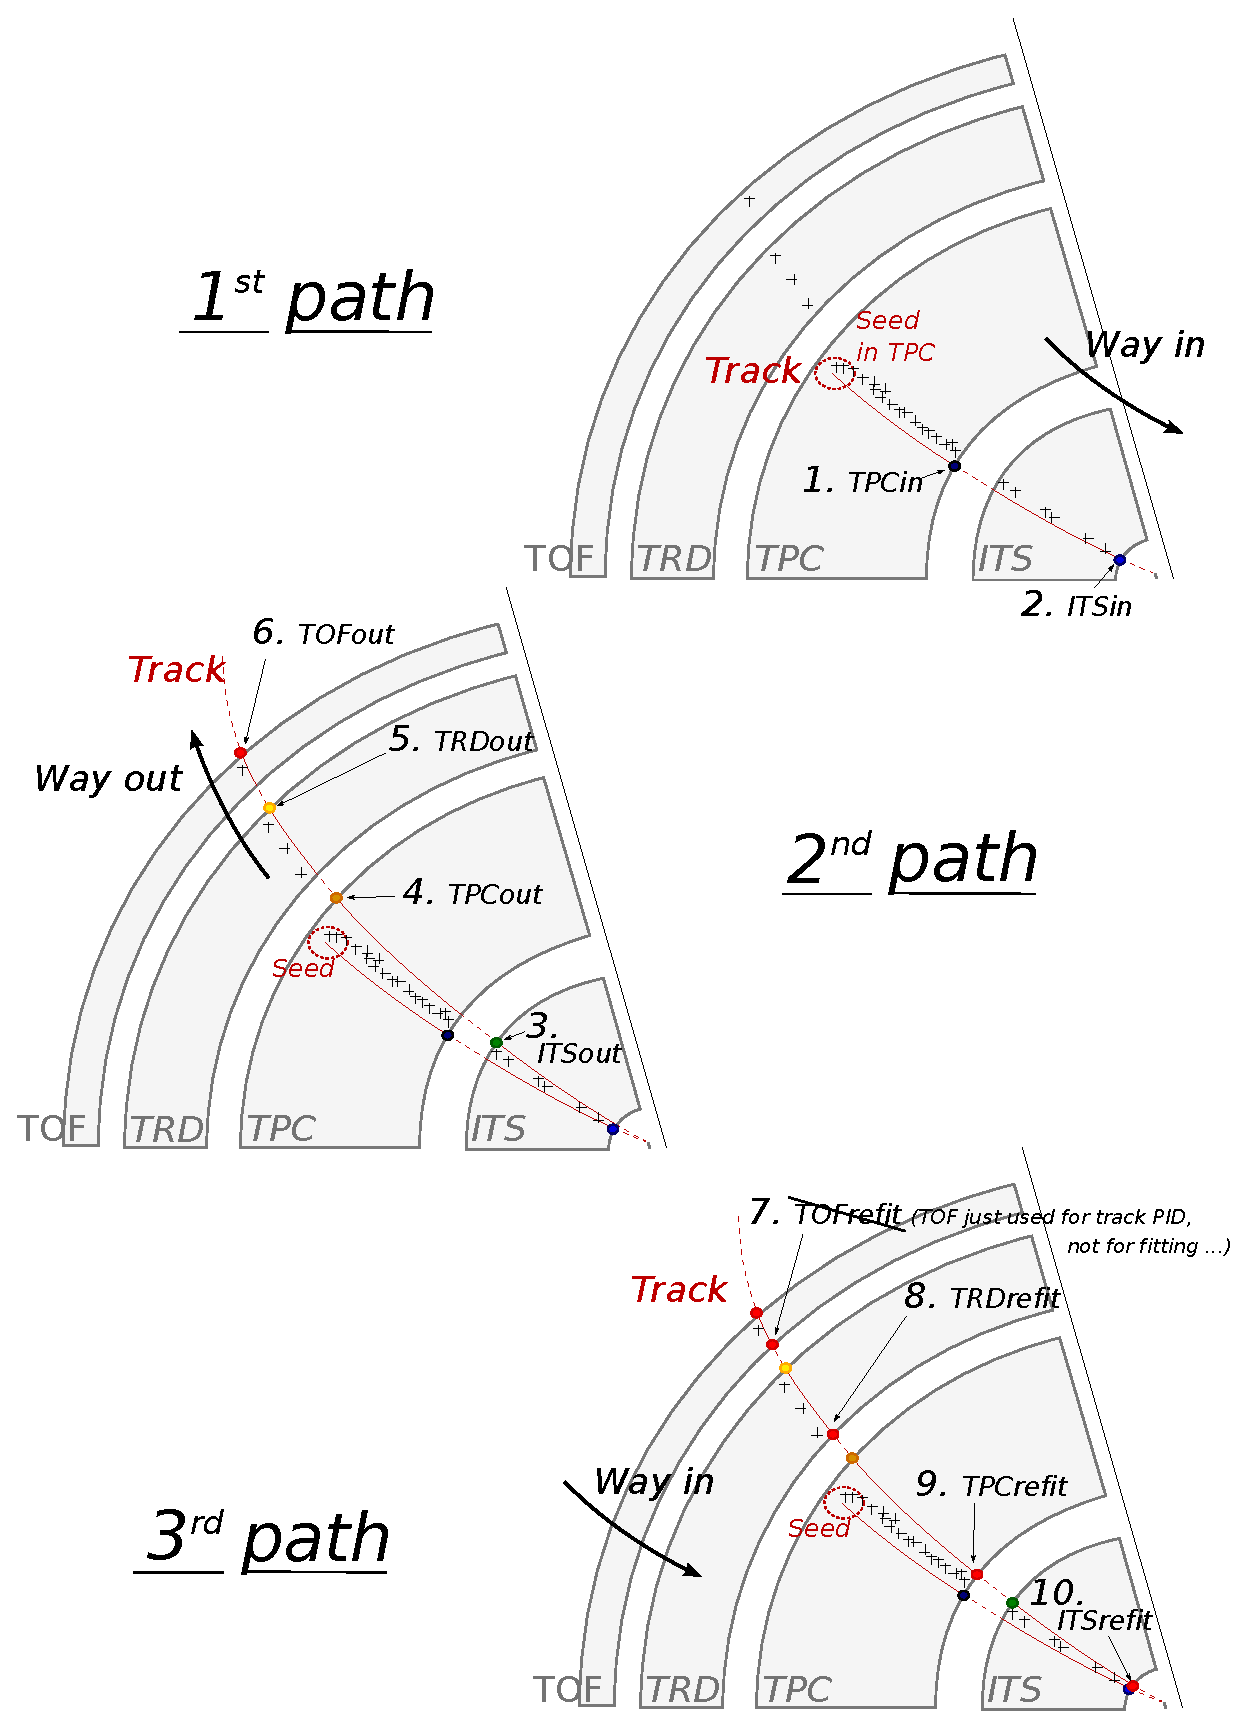
\includegraphics[width=1.05\textwidth]{Figs/Chapter3/Schema-PcpTrackingALICE.eps}
	\caption{Overview of the different elements of the track reconstruction in ALICE, at each pass of the Kalman filter. Figure taken from \cite{maireTrackReconstructionPrinciple2011}.}
	\label{fig:Kalmanfiltering}
\end{figure}

During this propagation, a preliminary particle identification based on the energy deposit in the TPC gas (see \Sec\ref{subsubsec:TPC}) allows to determine the most probable mass of the track candidate among eight hypothesis: \ePlusMinus, \muPlusMinus, \rmPiPlusMinus, \Kplusmin, \pOrPbar, \rmDeutonPM, \rmTritonPM, \rmHeThreePM or \rmHeFourPM. In cases where there is an ambiguity, the pion mass is assigned by default. From this and the amount of crossed material at each step, energy losses can be corrected on average using the Bethe-Bloch formula (\eq\ref{eq:BetheBloch}). It should be emphasised that all the parameters related to the TPC corresponds, in fact, to those of Ne. This approximation is justified by i) the fact that the TPC gas consists mainly of this element (until 2017), and ii) the effect is relatively small. 

When all the seeds have reached the inner wall of the TPC, the tracking in the ITS takes over. The reconstructed TPC tracks are extrapolated from the TPC inner wall ($\sim 85$ \cm) to the outermost layers of the ITS (38 and 43 \cm), that serve as seeds for the track finding in the ITS. Similarly as in the TPC, the seeding procedure produces two kinds of seed: first, one with vertex constraint, then the other without it. Whatever the hypothesis, they are all propagated as close as possible to the primary vertex, and updated along the way by any cluster passing a proximity cut. Only the highest quality candidates in the ITS from each TPC track are selected. A further check on cluster sharing among each other is performed. In such a case, the tracking algorithm tries to find another candidate and if this fails, the worst of the two tracks receives a special flag for containing a shared cluster, that is a potentially incorrectly assigned cluster.

Once all the ITS-TPC tracks have been formed, the ITS standalone tracking procedure comes into play and uses the remaining clusters to recover unfound tracks in the TPC because of i) their very low momentum or ii) the deadzones between sectors, or iii) decays before reaching the chamber. Formed out of two clusters from the three innermost layers and the preliminary vertex point, the seeds are propagated to the other layers, and updated with clusters passing a proximity cut. Only the track hypothesis with the smallest reduced $\chi^{2}$ is kept, and its assigned clusters are removed from further track finding. The procedure repeats until there are no more track to search. 

Upon completion of the track reconstruction in the ITS, the first stage of the tracking ends with the extrapolation of all tracks to their point of closest approach to the preliminary primary vertex. As in the TPC, energy loss corrections are applied at each propagation step in the ITS, considering the same mass hypothesis as one used previously and assuming that all the materials in the ITS volume (including the beam pipe) are made of Si\footnote{This relies on the same reasons as the ones mentionned in the case of the TPC. The \chap\ref{chap:CPTAnalysis} will showcase the limits of this approximation.}.\\

The second stage starts with the outwards propagation from the primary interaction point to the outermost layers of the ITS, and then towards the TPC outer wall (second path on \fig\ref{fig:Kalmanfiltering}). Based on the track parameters from the first iteration, the Kalman filter goes in the outward direction through the previously associated clusters. This also allows to calculate the track length integral, as well as the expected time of flight for the eight particle mass hypothesis, which are updated at each step. When reaching the outer edge of the TPC, the Kalman filter stops updating the track parameters but continues the propagation further detector (TRD, TOF, EMCal, PHOS, HMPID) for to hit matching. The track length integration and time-of-flight calculations terminates upon arriving at the TOF detector. \\

At the final stage (third path on \fig\ref{fig:Kalmanfiltering}), starting from the TPC outer wall, all tracks are propagated inwards to their distance of closest approach (DCA) to the preliminary primary vertex. Along the way, their parameters are improved one last time with the previously associated clusters in each detector. \\

\begin{figure}[t]
	\centering
	\includegraphics[width=0.9\textwidth]{Figs/Chapter3/PTresolution_vs_1Pt_pPb_2013_PerfPaper-8441.png}
	\caption{Transverse momentum resolution for TPC standalone and ITS-TPC combined tracks, with and without vertex constraint, as a function of $1/\pT$ in p-Pb collisions at \sqrtSnn = 5.02 \tev. The blue squares can not be seen as they overlap withe green ones. Figure taken from \cite{alicecollaborationPerformanceALICEExperiment2014}.}
	\label{fig:MomResolution}
\end{figure}

The reconstruction efficiency of TPC standalone tracks saturates around 80-85\% for transverse momentum above 0.5 \gmom, due to the loss of clusters in the deadzones between sectors. At lower \pT, it drops rapidly because of the dominance of multiple scattering and energy loss in the detector material. Whatever the detector occupancy, the contamination of wrongly associated clusters in the TPC remains low; it does not exceed 3\% for tracks with more than 10\% of fake clusters, even in the most violent heavy-ion collisions.

The TPC track prolongation efficiency to the ITS shows little dependence on the transverse momentum. It reaches $\sim$ 95\% for tracks with at least two associated hits in the ITS, and decreases to about 80\% in pp collisions at \sqrtS = 7 \tev (75\% in Pb-Pb collisions at \sqrtSnn = 2.76 \tev) when they have a minimum of one hit over two SPD layers, the furthest detectors relative to the TPC. The contamination of wrongly associated ITS clusters, though, can be quite high: $\sim$ 30\% of tracks with at least one fake cluster below $\pT < 0.2$ \gmom, $\sim$ 7\% at 1 \gmom, and below 2 \% at 10 \gmom in the most central Pb-Pb collisions.

The \fig\ref{fig:MomResolution} shows the resolution on the inverse transverse momentum for TPC standalone and ITS-TPC combined tracks, extracted from their covariance matrix. This quantity is related to the relative transverse momentum resolution, $\sigma_{\pT}/\pT$, via 
\begin{equation}
\sigma_{1/\pT} = \frac{\sigma_{\pT}}{\pT} \frac{1}{\pT} \quad \Rightarrow \quad \frac{\sigma_{1/\pT}}{1/\pT} = \frac{\sigma_{\pT}}{\pT}.
\end{equation}
In general, the transverse momentum resolution varies as a function of the transverse momentum; typically, it is at least as good as 0.9\% at $\pT = 1$ \gmom and 6\% at $\pT = 10$ \gmom. Note that the global ITS-TPC tracks always yields to a better relative \pT resolution than those reconstructed only with the TPC. In the latter case, the vertex constraint on the seeding strongly improves the resolution but the effect is negligible with a matching to the ITS detectors.


\subsubsection{Final determination of the primary vertex}

The end of tracking stage initiates a new determination of the primary vertex, based on the ITS-TPC combined tracks. Unlike the tracklets, their curvature is known, which allows to find the interaction point with a much higher precision.\\

All the global tracks are extrapolated as close as possible to the nominal beam position (or luminous region\footnote{When two beams collide, it gives rise to one or multiple collisions. Their interaction point \textit{a priori} lies anywhere within the region defined by the convolution of the particle distribution -- in other words, the beam size -- of the two incoming beams. Also called \textit{interaction region}, its transverse size is given by $\sigma_{D} = \sigma^{\rm beam} / \sqrt{2}$ \cite{carminatiALICEPhysicsPerformance2004}.}). After rejection of far outliers, the approximate point of closest approach of all selected tracks provides a first estimation of the interaction vertex. From here, in the near vicinity of its true position, a highly precise vertex fit can be performed \cite{karimakiEffectiveVertexFitting1997}. It basically consists in finding the space point that minimises the weighted\footnote{The track weighting has the effect of suppressing the contribution of any remaining outliers.} distance of closest of approach to this same point over all the tracks, as in \eq\ref{eq:SPDVertexer}. 

The precision on the vertex position increases with the number of tracks employed in the fitting algorithm. Therefore, in low-multiplicity events, the fit also includes the nominal beam position as an additional constraint/contribution with an uncertainty corresponding to the transverse size of the luminous region \cite{karimakiEffectiveVertexFitting1997}. Although high-multiplicity events have plenty of tracks available, the high pile-up rate requires a different approach. In order to reduce the contamination from collisions, only tracks coming from the same bunch crossings (identified thanks to the time information measured in the TOF detectors) can contribute to the same vertex. To further suppress the contribution of outliers, the vertex fitting relies on a more robust technique based on Tukey bisquare weights \cite{alicecollaborationPerformanceALICEExperiment2014}. \\

The \fig\ref{fig:VertexResol} shows the transverse resolution on the primary vertex position as a function of the particle multiplicity per unit pseudo-rapidity in pp at \sqrtS = 7 \tev. As mentioned above, the accuracy on the interaction point position sharply improves with the track multiplicity in the event, reaching $\sim 50$ \mum for $\dNdeta > 15$. With respect to the preliminary vertices found with the SPD tracklets, the final ones determined with global tracks is better by at least a factor of two. Note that both resolutions scale as the square root of the number of contributing tracks/tracklets \cite{caffarridavideCharmSuppressionPbPb2012}.

\begin{figure}[t]
	\centering
	\includegraphics[width=0.9\textwidth]{Figs/Chapter3/VertexRes-8462.png}
	\caption{Transverse width of the final vertex distribution, in solid markers, in pp collisions at \sqrtS = 7 \tev. Two contributions are separated: the transverse size of the nominal beam position $\sigma_{\rm D}$, and the transverse resolution on the vertex $\alpha / \sqrt{ \left( \dNdeta \right)^{\beta} }$. For comparison, the open markers show the same quantity determined making use of SPD tracklets. Figure taken from \cite{alicecollaborationPerformanceALICEExperiment2014}.}
	\label{fig:VertexResol}
\end{figure}

\subsection{The ALICE offline framework}

\subsubsection{The computing model}

Over the whole LHC Run-2, more than 160 PB of raw data have been collected by the ALICE experiment. Their treatment requires a robust framework, capable of processing them in a reliable and timely fashion. 

To be processed, this volume of data requires an amount of computing resources that can not be concentrated in one place\footnote{There are various reasons. Although the funding agencies invest in the computing equipment of their scientific projects, they focus their investments in their own countries. Even if all computing resources could be put in one place -- let us say, at CERN --, the manpower would be insufficient to ensure the upkeep of such a system.}. Instead, it is spread over different computing centres around the world. In particular, ALICE uses the Worlwide LHC Computing Grid (WLCG), a worldwide computer network infrastructure coordinated by the CERN and shared among all LHC experiments, that includes over 170 computing centres in 42 countries. The WLCG stands as the world's largest computing grid, that provides near real-time access to the LHC data regardless of their physical location \cite{worldwidelhccomputinggridWorldwideLHCComputing}.

\begin{figure}[b]
	\centering
	\includegraphics[width=0.8\textwidth]{Figs/Chapter3/WLCG-Tiers-2021_v3_1.png}
	\caption{The three Tiers of the Worlwide LHC Computing Grid as of 2023, with the list of the thirteen Tier-1 computing centres, with their geographic location. Figure taken from \cite{worldwidelhccomputinggridWorldwideLHCComputing}.}
	\label{fig:WLCG}
\end{figure}

The WLCG computing sites follows a hierarchical structure in layers or \textit{Tiers} as shown in \fig\ref{fig:WLCG}, that provides different levels of data storage and processing. The Tier-0 corresponds to the CERN Data Centre located in Geneva, that directly receives all the raw data from the LHC experiments, keeps one replica (on magnetic tapes) and performs the first reconstruction pass. It also distributes the raw data and the reconstruction output to the thirteen Tier-1 computer centres around the world via high-speed connections between 10 and 100 GB/\second. They share the same roles with CERN, namely safe-keeping the data, finishing their reconstruction and distributing them to the next layer. The Tier-2 regroups about 160 sites, corresponding typically to universities and scientific institutes, that store the data produced by the closest Tier-1 site. Beyond their mass-storage capabilities, they are used to run the physics analysis tasks, produce Monte Carlo simulations, and reprocess the data. A copy of the simulated data is stored in the Tier-1 centres.

Each site relies on four components: networking, hardware, middleware and physics analysis software. The networking -- the backbone of any distributed computing infrastructure -- allows to link together the hundreds of WLCG centres and exchange data with an excellent connectivity thanks to the CERN Internet Exchange Point, the high-bandwidth LHC optical-fibres and the Grid File Transfer Service. Each site can be seen as computer farm that needs tending to; the hardware component refers to this aspect. It includes maintaining disk and tape servers, providing tools to access the data whatever the storage medium --- via the \textbf{C}ERN \textbf{A}dvanced \textbf{STOR}age system (CASTOR) or CERN EOS --- as well as upgrading regularly the necessary software to operate the Grid system --- from the operating system to the physics analysis software libraries. The middleware corresponds to the software architecture that comes between the operating systems and the physics analysis software; it provides numerous services (interfacing, workload management, monitoring, job submission and execution, etc) in order to access at the titanic CPU power and storage ressources of the Grid. In ALICE, the AliEn system fill in this task. Last but not least, the physics analysis software provides the tools to analyse the data.


\subsubsection{The analysis framework, AliRoot}
\label{subsubsec:AliRoot}

As most of the current high-energy experiments -- if not all --, the ALICE offline analysis framework is built upon ROOT, an high-performance object-oriented software developed by the CERN and implemented almost entirely in the C++ programming language. Created in 1994 by René Brun and Fons Rademakers, it provides the mathematical and statistical tools to manipulate large amounts of data and analyse them \cite{renebrunandfonsrademakersROOTObjectOriented}. ROOT sets the foundation for the ALICE offline framework, that divides into two parts during the LHC Run-1 and Run-2:
\begin{itemize}
\item[$\ $] \textbf{AliRoot} \cite{alicecollaborationAliRoot} contains the codes that are common to the whole collaboration. In particular, it includes:
\begin{itemize}
\item[$\bullet$] an interface for running Monte Carlo simulations (from the event generation to the detector response), event visualisation, etc,
\item[$\bullet$] a description of the detector geometry as well as the material budget,
\item[$\bullet$] the alignement and calibration of the detectors, 
\item[$\bullet$] the real and simulated data reconstruction,
\item[$\bullet$] and the management of the data formats;
\end{itemize}
\item[$\ $] \textbf{AliPhysics} \cite{alicecollaborationAliPhysics2023} regroups all the physics analysis tasks to process the collected and simulated events. Each PWG (\tab\ref{tab:PhysicsBoard}) has a dedicated repository.
\end{itemize}

\subsubsection{Data formats}
\label{subsubsec:DataFormats}

Depending on the processing stage, the ALICE data come in three distinct formats with different level of abstraction. At the output of the detectors (\Sec\ref{subsec:ALICEDetector}), they take the form of \textit{Raw Data}, that regroups all the cluster informations recorded during a collision. They are collected by the DAQ system before being transmitted at a rate of 200 MB/\second to the Tier-0 site for storage and distribution to Tier-1 data centres. 

In parallel, the raw data undergo their first reconstruction pass at CERN. For pp collisions, it typically takes two minutes per event in pp collisions, mainly in input/output streaming. This first pass yields to an Event Summary Data (ESD) format, that  contains most of the informations related to the reconstruction such as the reconstructed tracks with their associated hits. While an event from raw data occupies about 1 MB of disk space, it reduces to $\sim$ 100 kB in ESD format. 

At the analysis level, the ESD file presents the advantage of having the full knowledge of the tracking and event building, with the possibility of replaying some part of the reconstruction like the V0 and cascade vertexings (see next chapter, \chap\ref{chap:V0CascReconstruction}). However, they are still considered as too heavy and too expensive in terms of CPU time. For that reason, the first pass also produces a file in Analysis Object Data (AOD) format, a lighter version than the ESD counterpart, keeping only the relevant information to extract the physics content from the data. It covers 5 to 10 times less disk space than an ESD file, thereby reducing significatively the processing time by the analysis tasks.\\

Note that the first reconstruction pass only serves to calibrate the TPC, SDD, TOF, T0, luminous region and centrality. The second pass applies the derived calibration, and is then used to improve the calibrations and perform a first data quality assurance. These two reconstruction passes, using only a fraction of the data from each run, provides the input for a more complete and fine-tuned calibration, that is stored in the Offline Conditions DataBase\footnote{In fact, OCDB stores the ideal geometry of the detector,  the alignement objects (\ie corrections on the ideal geometry derived using Millepede algorithm \cite{blobelNewMethodHighPrecision2002}) and the calibration parameters for each data taking period.} (OCDB) and is applied in the third pass. At each stage of the processing, a set of ESD and AOD files is produced. 

\subsubsection{Monte Carlo data}
\label{subsubsec:MCData}

As mentionned in \Sec\ref{subsubsec:AliRoot}, the AliRoot framework has the capability to run Monte Carlo (MC) simulations, that try to reproduce as accurately as possible the stochastic processes observed in the detector by sampling a given set of probability density distributions. Such a simulation consists in two consecutive steps.

It starts with the generation of the event, that simulates a collision as well as the associated physics processes ultimately leading to the creation of primary particles. This first step relies on different models called \textit{event generators}, each having its own paradigm, its own production mechanisms, tuned to mimic the topology the collision (multiplicity, momentum distribution, etc). Among the most commonly used, there are \Pythia \cite{bierlichComprehensiveGuidePhysics2022} and \Herwig \cite{bahrHerwigPhysicsManual2008} for pp collisions, \Epos \cite{pierogEPOSLHCTest2015} for both pp and heavy-ion collisions, \Hijing \cite{wangHIJINGMonteCarlo1994} exclusively for heavy-ion collisions.

After the generation of the event comes the propagation of the primary particles through the ALICE detector. This requires a modelisation of the apparatus in its entirety, from the various elements composing the sub-detectors to their geometric shape and their positioning. It also has to account for noisy or dead channels, detector defects, intensity of the magnetic field, etc. These informations available run by run on OCDB are used to \textit{anchor} the simulation on the data taking conditions. The transport and interaction with the detector material typically rely on softwares, such as \GeantThree \cite{brunGEANTUserGuide1987}, \GeantFour \cite{geant4Geant4HomePage} and \Fluka \cite{battistoniOverviewFLUKACode2015}.

Taking into account the detector response, the energy deposited by the passage of charged particles are converted into digits and then stored in raw data format. From this point, the reconstruction of the event can start. It follows the same procedure as the one applied for real data (\Sec\ref{subsec:EventReco}), yielding to files in ESD and AOD formats.

In order to minimise the disk space usage and the computing time, only a fraction of the total number of events in real data is simulated. The proportion of triggers remains unchanged between real and simulated data, though. For instance, if a run in its entirety has 10\% of high-multiplicity events, its simulated twin will comprise the same fraction of such events.\\

The key point of MC data resides in the presence of the full information about the event. This is often referred as \textit{MC truth}. Each element of the simulation is perfectly known: the number of generated particles, their type, charge, momenta, whether they are primary or secondary, where they deposit energy in the detector giving rise to hits -- the so-called track references --, etc. This copious amount of additional informations opens the door to other kinds of investigations. 

When designing a new experiment, it allows to anticipate the results and, if needed, to correct or optimise the current design. It gives also the opportunity to estimate the performances of a detector (typically, the efficiency) and to study its systematic features. Finally, the comparison between the measurements (real data) and the predictions from a given MC model (simulated data) helps to improve our understanding of the underlying physics.\\

It should be mentionned that there exists two classes of MC simulations in high-energy physics. Reproducing as accurately as possible a collision requires tuning the parameters of the simulation such that they correspond to the ones observed in real data, including the decay channels, the branching ratios, etc. This is the standard type of simulations, the \textit{general-purpose} MC production. A limitation arises from rare signals: for them to be observed, an unrealistic amount of events would need to be generated. 

Instead, one could resort to an \textit{enriched} MC simulations, in which the abundancy of rare signals is increased. This can be achieved by artificially injecting the particles of interest in the simulation, according to a flat distribution in \pT or rapidity, etc. Another option consists in embedding a pure sample of rare signals into a background event, coming from either a simulation or real data. This is particularly used in p-Pb or Pb-Pb simulations, where \Pythia -- a generator dedicated to pp collisions -- produces an event with an enhanced abundancy in rare signals. However, the topology of the simulated event does not coincide with the one in p-Pb or Pb-Pb collisions. Therefore, the injected event is incorporated into a \Hijing event, that plays the role of a background event\footnote{Note that the background event can \textit{a priori} be re-used several times.}.